\section{Introduction}

%%Introducing codon models and their usefulness
Phylogenetic codon models are now routinely used in many domains of bioinformatics and molecular evolutionary studies.
One of their main application has been to characterize the genes, sites~\citep{Nielsen1998}, or lineages~\citep{Zhang2004} having experienced positive selection.
More generally, these models highlight the respective contributions of mutation, selection, genetic drift and biased gene conversion~\citep{Kosiol2019}, and the causes of their variation between genes~\citep{Zhang2015} or across species~\citep{Lartillot2011}.

%introducing the idea of a single $\omega$
Conceptually, codon models take advantage of the fact that synonymous and non-synonymous substitutions are differentially impacted by selection.
Assuming synonymous mutations are neutral, the synonymous substitution rate is equal to the underlying mutation rate~\citep{kimura1983neutral}.
Non-synonymous substitutions, on the other hand, reflect the combined effect of mutation and selection~\citep{Ohta1995}.
Classical codon models formalize this idea by invoking a single parameter $\omega$, acting multiplicatively on non-synonymous substitutions rates~\citep{Muse1994, Goldman1994}.
Using a parametric model automatically corrects for the multiplicity issues created by the complex structure of the genetic code and by uneven mutation rates between nucleotides.
As a result, this parameter $\omega$ capture the net, or aggregate, effect of selection on non-synonymous mutations.

%elaborating on the phenomenological versus mechanistic, classical versus mutsel, distinction
Classical codon models, so defined, are phenomenological, in the sense that they capture a complex mixture of selective effects through a single parameter~\citep{Rodrigue2010a}.
In reality, the selective effects associated with non-synonymous mutations depend on the context (site-specificity) and the amino acids involved in the transition~\citep{Kosiol2007}.
Attempts at an explicitly modelling of these complex selective landscapes have also been done, leading to mechanistic codon models, based on the mutation-selection formalism~\citep{Halpern1998}.
These models, further developed in multiple inference frameworks~\citep{Rodrigue2010, Tamuri2012}, sometimes using empirically informed fitness landscapes~\citep{Bloom2014}, could have many interesting applications, such as inferring the distribution of fitness effects~\citep{Tamuri2012} or detecting genes under adaptation~\citep{Rodrigue2016}, or even phylogenetic inference.
However, they are computationally complex and potentially sensitive to the violation of their assumptions about the fitness landscape (such as site independence).
For that reason, classical codon models remain an attractive, potentially more robust, although still perfectible, approach.

%bringing in the key issue here: correctly teasing apart mutation and selection
The parametric design of current classical models, relying on a single aggregate parameter $\omega$, raises the question whether they reliably estimate the underlying mutational process.
several observations suggest that this may not be the case.
For instance, in their simplest form~\citep{Muse1994, Goldman1994}, classical codon models predict that the nucleotide composition should be the same for all three positions of the codons, and should be equal to the nucleotide equilibrium frequencies implied by the underlying nucleotide substitution rate matrix.
In reality, the nucleotide composition differs: the third position shows more extreme composition, reflecting the underlying mutation bias, compared to first and second positions, which are typically closer to 50\% GC~\citep{Singer2000}.

These modulations across the three coding positions have been accommodated using the so-called 3x4 formalism~\citep{Goldman1994, Pond2005a}, allowing for different nucleotide rate matrices at the three coding positions.
However, this is also problematic, since this modelling approach has the consequence that synonymous substitutions, say, from A to C, occur at different rates at the first and third positions.
Yet, in reality, the mutation process is blind to the coding structure, and should be homogeneous across coding positions, and if neutral, all mutations from A to C should thus have the same rate.

%Potential impact of these problems: both practical and conceptual
These observations suggest that the mutation matrix (1x4) or matrices (3x4) estimated by codon models are not correctly reflecting the mutation rates between nucleotides~\citep{Rodrigue2008a}.
Instead, what these matrices are capturing is the result of the compromise between mutation and selection at the level of the realized nucleotide frequencies.
For detecting selection, this problem is probably minor, although it still bears consequences on the estimation of $\omega$~\citep{Spielman2015}.
Conceptually, however, it is a clear symptom of a more fundamental problem: mutation rates and fixation probabilities are not correctly teased apart by current codon models.

Practically, this misconception could have important consequences in other contexts than tests of positive selection.
In particular, there is a current interest in investigating the variation between species in GC content, and its effect on the evolution of protein-coding sequences~\citep{Bolivar2019}.
An important factor here is biased gene conversion toward GC (called gBGC), which can confound the tests for detecting positive selection and, more generally, the estimation of $\dnds$~\citep{Galtier2009,Ratnakumar2010, Figuet2014}.
Even in the absence of \acrshort{gBGC}, however, uneven mutation rates varying across species can have an important impact on the estimation of the strength of selection.
All this suggests that, even before introducing \acrshort{gBGC} in codon models, correctly formalizing the interplay between mutation and selection in current codon models would be an important first step.

%The mut-sel balance revisited: an equilibrium between two net forces
In this direction, the key point that needs to be correctly formalized is the following.
If the nucleotide's realized frequencies are the result of a compromise between mutation and selection, then this implies that the strength of selection is not the same between all nucleotide or amino-acid pairs.
For instance, if the mutation process is AT-biased, then, because of selection, the realized nucleotide frequencies at equilibrium will be less AT-biased than expected under the pure mutation process.
However, this implies that, at equilibrium, there will be a net mutation pressure toward AT, which has to be compensated for by a net selection differential toward GC.
In other words, at equilibrium, mutations toward AT will be more deleterious on average than those toward GC, or equivalently, the $\dnds$ toward AT will be lower than the $\dnds$ toward GC.

%introducing $\omega$ as a tensor
All this suggests that, in order for a codon model to correctly formalize this subtle interplay between mutation and selection, the component of the parameter vector responsible for absorbing the net effect of selection (i.e.~$\omega$) should not be a scalar, as is currently the case.
Instead, it should be a tensor, that is, an array of $\omega$ values unfolding along multiple directions.
In the present work, we address the question of whether we can derive a parametric structure being able correctly tease apart mutation rates and selection, and this, without having to explicitly model the underlying fitness landscape.
In order to derive a codon model along those lines, our strategy is to first assume a true site-specific evolutionary process, following the mutation-selection formalism.
Then, we derive the mean substitution process implied across all sites by this mechanistic model and identify the mean fixation probabilities appearing in this mean-field process with the $\omega$ tensor to be estimated.
Inferring parameters on simulated alignments, we show that the model correctly estimates the mutation rates, as well as the mean effect of selection and its modulations in the different nucleotide directions.

% Improved inference of site-specific positive selection under a generalized parametric codon model when there are multinucleotide mutations and multiple nonsynonymous rates~\citep{Dunn2019}.
% Influence of mutation bias and hydrophobicity on the substitution rates and sequence entropies of protein evolution~\citep{Santos2018}.


\section{Results}
\label{sec:results}

To illustrate the problem, we first conduct simulation experiments under a simple mutation-selection substitution model assuming site-specific amino-acid preferences.
We use these simulation experiments to explore through summary statistics the intricate interplay between mutation and selection.
Then, we explore how codon models with different parameterizations are able to infer the mutation rates and the strength of selection on these simulated alignments.
Finally, these alternative models are applied to empirical data.

\subsection{Simulations experiments}
\label{subsec:simulations-experiments}

Simulations of protein-coding \acrshort{DNA} sequences were conducted under an origination-fixation substitution process~\citep{McCandlish2014} at the level of codons (see section~\ref{sec:mut-bias-simu}).
We assume a simple mutation process with a single parameter controlling the mutational bias toward AT, denoted $\lambda = (\mutequi_A+\mutequi_T)/(\mutequi_C+\mutequi_G)$, where $\mutequi_x$ is the equilibrium frequency of nucleotide $x$.
This mutational process is shared by all sites of the sequence.
With regards to selection, synonymous mutations are considered neutral, such that the synonymous substitution rate equal to the underlying mutation rate.
At the non-synonymous level, selection is modelled by introducing site-specific amino-acid fitness profiles (i.e.~a vector of 20 fitnesses for each coding site), which are drawn from a uniform dirichlet distribution of concentration parameter $\alpha$.
A low $\alpha$ induces site-specific profiles having a large variance, with some amino acids with a high fitness while all other have a low fitness.
Conversely, a large value for $\alpha$ induces more even amino-acid fitness profiles at each site.
Thus, ultimately, the stringency of selection increase with decreasing $\alpha$.
Altogether, the two parameters of the model tune the mutation bias ($\lambda$) and the stringency of selection ($\alpha$), respectively, as depicted in figure~\ref{fig:mut-bias-parameters}.
All simulations are obtained using the same underlying topology of 180 species and 498 codon sites.

\begin{figure}[htbp]
    \centering
    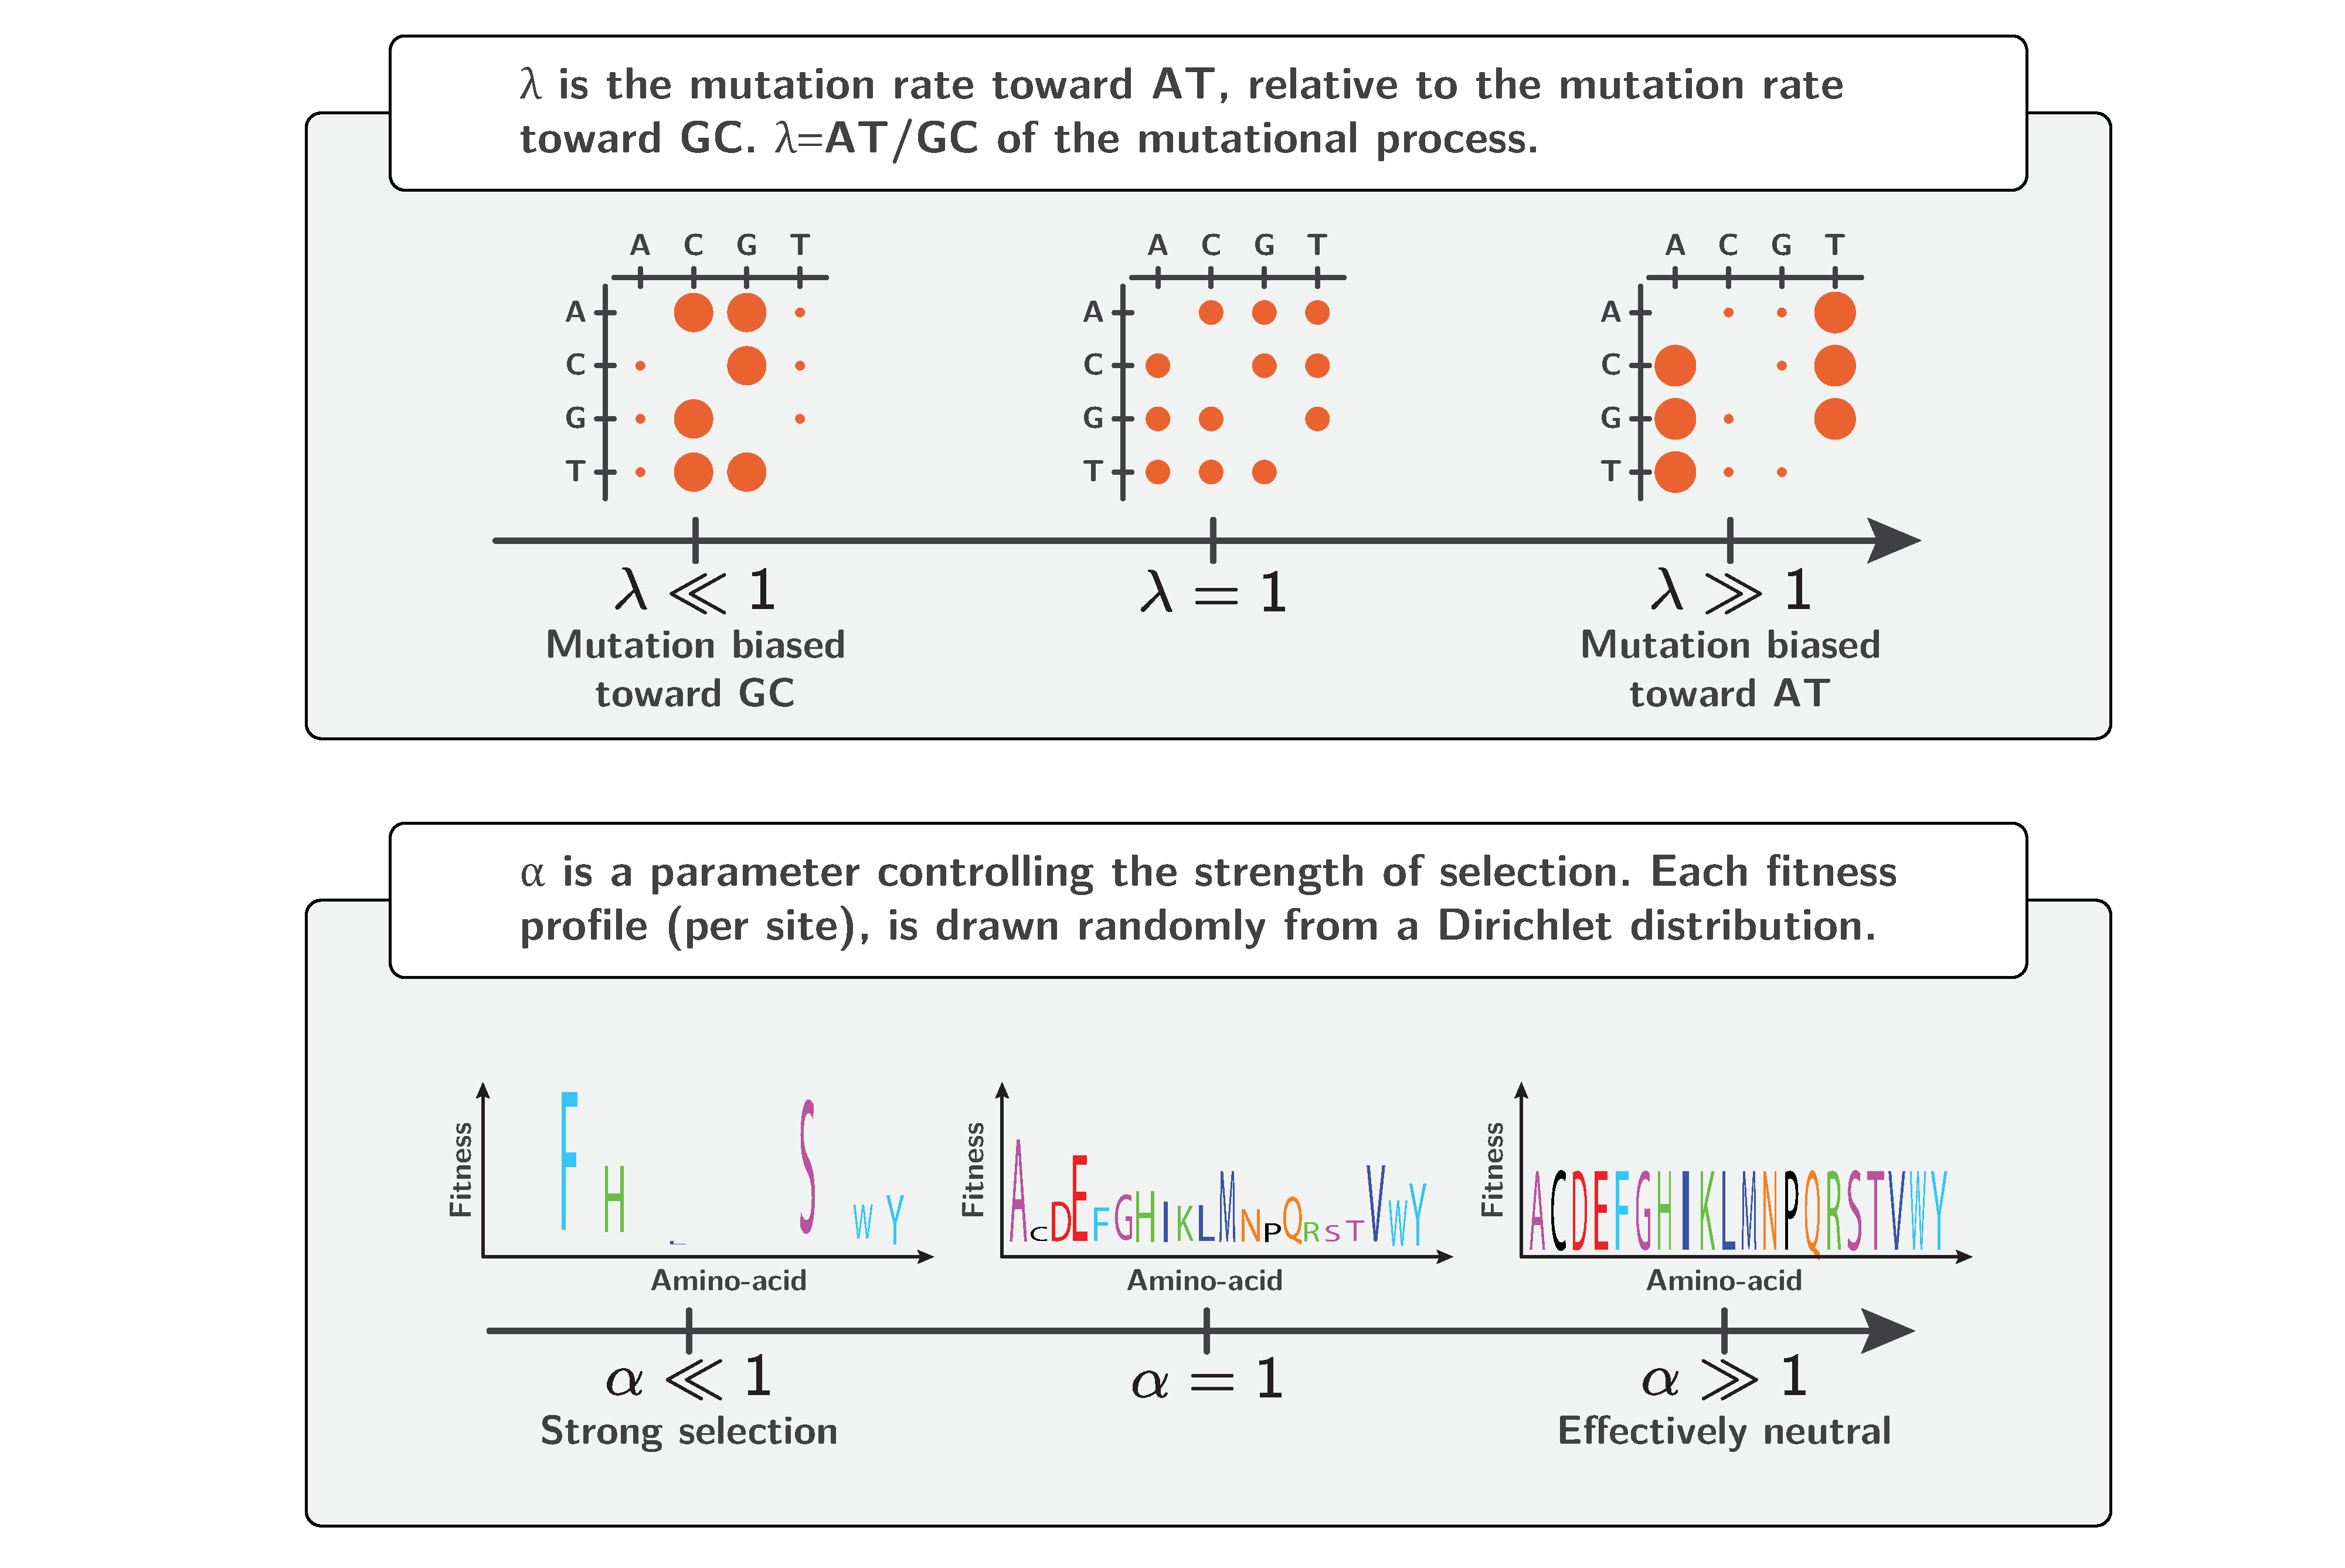
\includegraphics[width=\textwidth] {parameters}
    \caption[Parameters of the mutation-selection model]{
    Parameters of the mutation-selection model.
    Mutational bias (toward A and T) is shared by all sites of the sequence, and tuned by the parameter $\lambda$.
    Conversely, each codon site of the sequence is defined by a unique fitness profile, drawn from a Dirichlet distribution with concentration parameter $\alpha$.
    Stringency of selection increase with decreasing $\alpha$.}
    \label{fig:mut-bias-parameters}
\end{figure}


Simulation of this origination-fixation process along a species tree result in a multiple sequence alignment of coding sequences for the extant species, from which summary statistics can then be computed.
One such straightforward summary statistic is the frequency of the different nucleotides, and the resulting nucleotide bias $\atgc$ observed in the alignment.
This observed nucleotide bias can be computed separately for each coding position (first, second and third) and compared to the underlying true mutational bias $\lambda$.
As can be seen from figure~\ref{fig:mut-bias-AT-GC-obs}, the third position of codons reflects the underlying mutational bias quite faithfully, while the first and second positions are impacted by the strength of selection and display nucleotide biases that are less extreme than the one implied by the mutational process.
This differential effect across the three coding positions is explained by nucleotide mutations at the third codon position being more often synonymous, while mutations at the first and second positions are more often changing the amino-acid and are thus more often under purifying selection.

\begin{figure}[htbp]
    \centering
    \begin{minipage}{0.32\linewidth}
        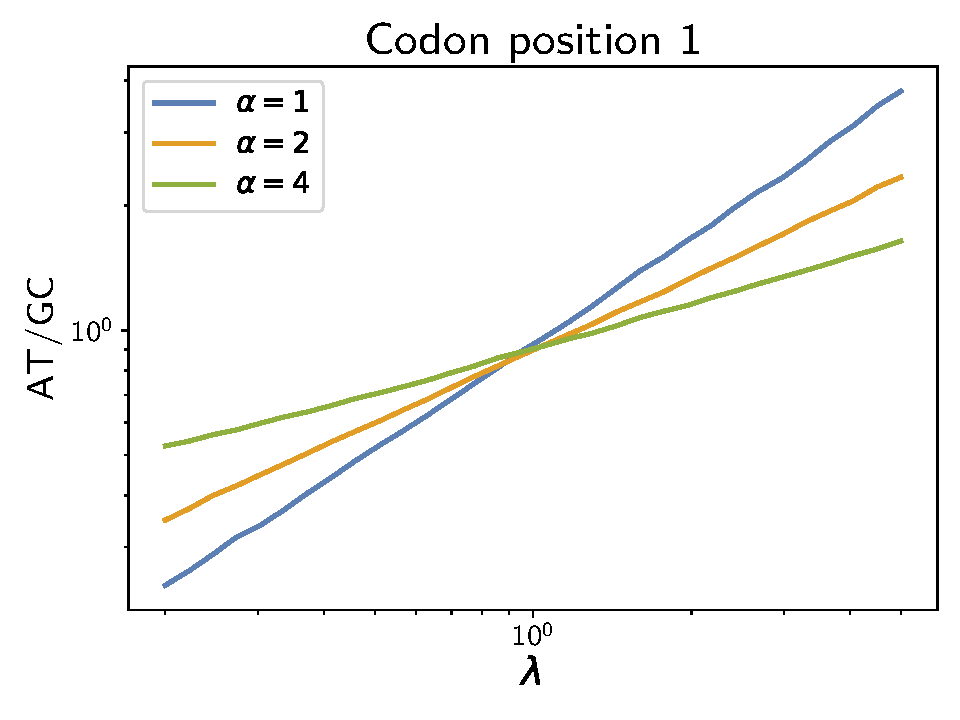
\includegraphics[width=\linewidth, page=1]{at_over_gc_1}
    \end{minipage}
    \llap{\raisebox{-1.0cm}{\scriptsize A\hspace{0.35cm}}}\hfill
    \begin{minipage}{0.32\linewidth}
        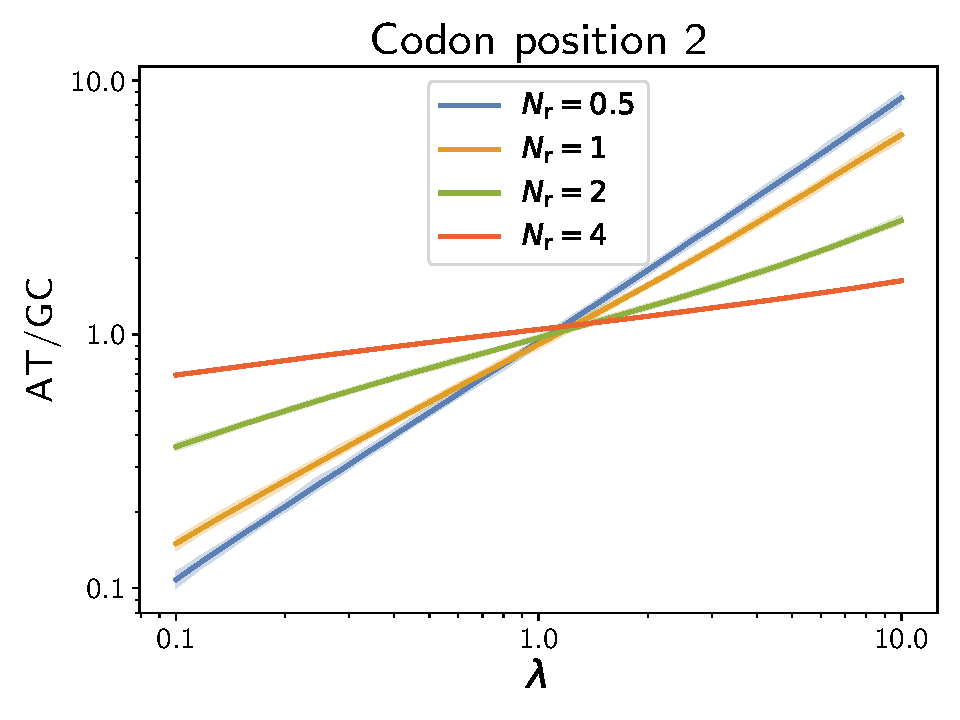
\includegraphics[width=\linewidth, page=1]{at_over_gc_2}
    \end{minipage}
    \llap{\raisebox{-1.0cm}{\scriptsize B\hspace{0.35cm}}}\hfill
    \begin{minipage}{0.32\linewidth}
        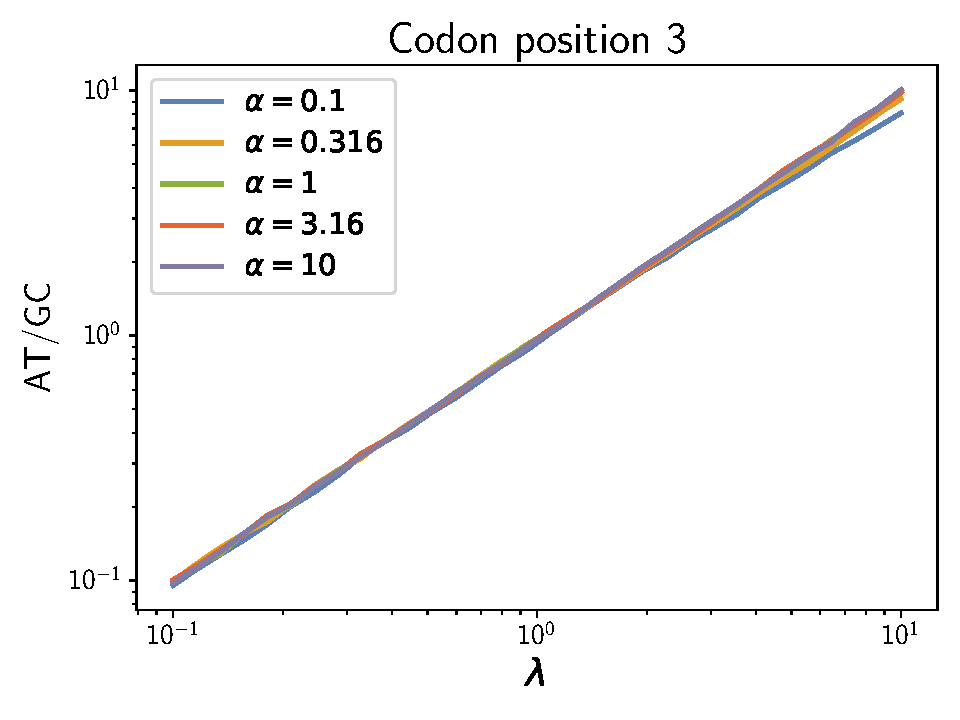
\includegraphics[width=\linewidth, page=1]{at_over_gc_3}
    \end{minipage}
    \llap{\raisebox{-1.0cm}{\scriptsize C\hspace{0.35cm}}}\hfill
    \caption[$\atgc$ composition of the alignment]{
    Observed $\atgc$ composition of the alignment, represented at the different positions of codons (first, second and third), summed over all sites.
    The horizontal axis represents the underlying mutational bias ($\lambda$) of the nucleotide matrix, and the vertical axis represent the observed $\atgc$ of the codon position across the alignment.
    Stringency of selection is represented by 5 coloured solid lines with decreasing $\alpha$.
    $\atgc$ at the third codon position (panel C) matches the mutational bias, whereas in contrast first and second positions (panel A and B) are less extreme than the underlying bias.
    With increase stringency of selection (i.e.~with decreasing $\alpha$), the observed bias is less reflecting the underlying mutational bias such that selection is opposing the mutational bias.}
    \label{fig:mut-bias-AT-GC-obs}
\end{figure}

Apart from the observed nucleotide bias in the alignment, the diversity of amino acids is an important indicator of the selective constraints that the sequence experiences.
This diversity can be quantified by the frequencies of amino acids observed across all taxa in the alignment, and then summarized through a single statistic, namely the Shannon entropy of amino-acid frequencies~\citep{Goldstein2017}, as described in section~\ref{subsec:entropy}.
Diversity can be quantified for a given site of the sequence, and this site-specific diversity can subsequently be averaged over all sites of the sequence (yielding what is hereafter called the site-specific diversity).
Alternatively, the diversity can be quantified directly on the amino-acid frequencies observed across the whole sequence alignment (which we refer to as the sequence diversity).

These two variants of the amino-acid diversity are computed for alignments simulated under different values of $\alpha$ and $\lambda$ (figure~\ref{fig:mut-bias-diversity-aa}).
Under stringent selection, only a small number of amino acids are typically permissible any given site, resulting in a low site-specific diversity.
Yet all amino acids occur at comparable frequencies in the alignment, resulting in a high sequence diversity.
These observations highlight the distinction between averaged site-specific diversity and global sequence diversity.
Of note, varying $\alpha$ has a strong impact on the site-specific diversity (figure~\ref{fig:mut-bias-diversity-aa}), directly reflecting the fact that more stringent selection amounts to reducing the number of acceptable amino-acids at each site.
On the other hand, it has a minor impact on sequence diversity, which merely reflects the fact that the strength of selection does not impact the global composition of the sequence.

Imposing a stronger mutational bias (either toward AT or toward GC) greatly reduces both site-specific and sequence diversity.
This shows that the composition in amino acids is highly dependent on the underlying mutational bias, but also, that a more extreme mutational bias results in a more constrained substitution process: in effect, under a strong mutational bias, only those amino-acids that have both a high fitness and codons enriched in the nucleotides favored by the mutational process are eventually observed.
This effect is less visible whenever selection is more stringent (i.e.~with decreasing $\alpha$), but can still be observed even for stringent selection.

\begin{figure}[htbp]
    \centering
    \begin{minipage}{0.49\linewidth}
        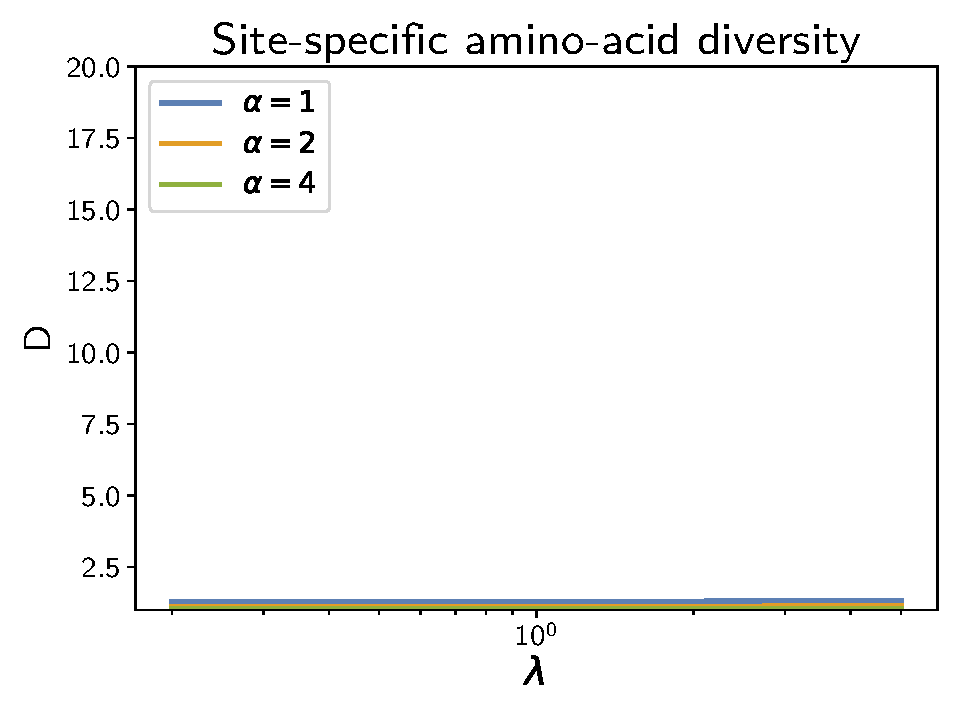
\includegraphics[width=\linewidth, page=1]{site_diversity_aa}
    \end{minipage}
    \llap{\raisebox{-1.6cm}{\scriptsize A\hspace{0.35cm}}}\hfill
    \begin{minipage}{0.49\linewidth}
        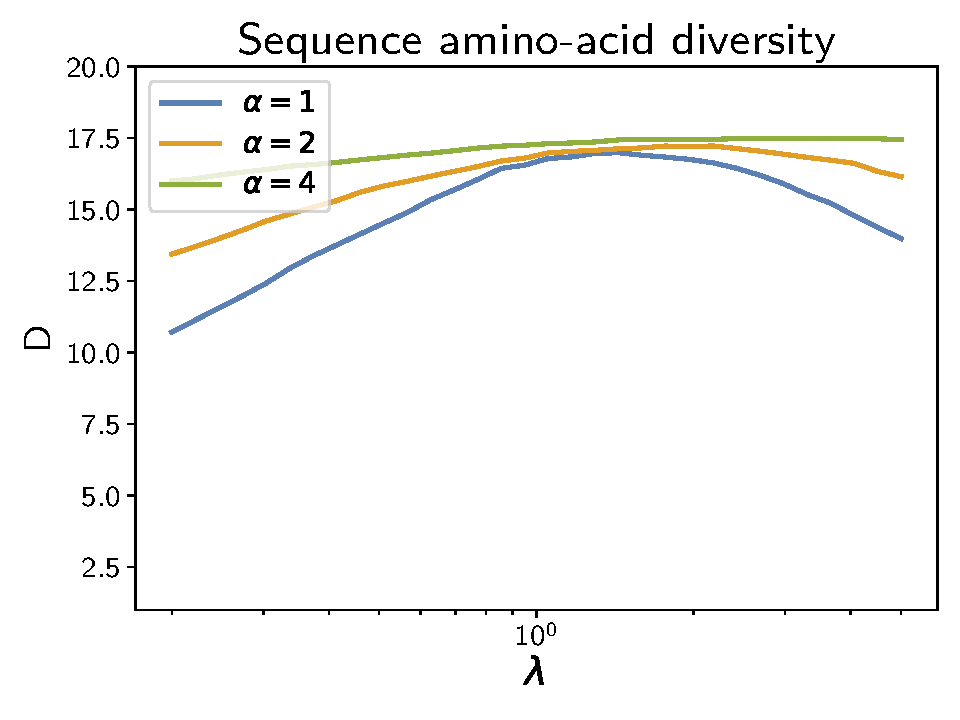
\includegraphics[width=\linewidth, page=1]{diversity_aa}
    \end{minipage}
    \llap{\raisebox{-1.6cm}{\scriptsize B\hspace{0.35cm}}}\hfill
    \caption[Diversity of amino acids]{
    Diversity of the amino-acid frequencies is quantified as the exponential of Shannon's entropy in the vertical axis, either as site-specific diversity in the panel A or as sequence diversity in the panel B.
    Sequence diversity is higher than site-specific diversity, because at any given site only a small number of amino acids are actually permissible.
    From a selective perspective, site-specific diversity decreases with stringency of selection (decreasing $\alpha$ represented by 5 different solid lines) because at given site only a few amino acids are permitted.
    Conversely, because site-specific fitness profiles are randomly drawn, each site has different permitted amino acid, increasing the sequence diversity as the stringency of selection increases.
    From a mutational perspective, diversity decreases with increased mutational bias toward either toward AT or GC ($\lambda$ in horizontal axis).
    This effect is explained by the high frequency of amino acids containing nucleotides favoured by the underlying mutational bias.
    Finally, under stringent selection, diversity is less sensitive to the underlying mutational bias.}
    \label{fig:mut-bias-diversity-aa}
\end{figure}

The observed diversity is the result of a mix between mutation and selection.
An alternative statistic, more directly relevant for measuring the intrinsic effect of selection, is the mean scaled fixation probability of non-synonymous mutations ($\avgpfix$).
This summary statistic $\avgpfix$ can be quantified from the substitutions recorded along the simulation trajectory (see section~\ref{subsec:fixation-bias}).
For very long trajectories, it identifies with the ratio of non-synonymous over synonymous substitution rates (or $\dnds$) induced by the underlying mutation-selection model~\citep{Spielman2015, DosReis2015, Jones2016}.
As expected, $\avgpfix$ is always lower than 1 for simulations at equilibrium, under a time-independent fitness landscape~\citep{Spielman2015}.
Quite expectedly (figure~\ref{fig:mut-bias-omega-WS}, panel A) $\avgpfix$ depends strongly on the stringency of selection ($\alpha$), which it is meant to measure.
On the other hand, $\avgpfix$ depends weakly on the mutational bias ($\lambda$).
This is in stark contrast with the amino-acid diversity, which is dependent on $\lambda$ (figure~\ref{fig:mut-bias-diversity-aa}).

The proxy of selection represented by $\avgpfix$ concerns all non-synonymous mutations, but we can also consider the mean scaled fixation probability only for the subset of non-synonymous mutations from weak nucleotides (A or T) to strong nucleotides (G or C), called $\avgpfix_{\ATtoGC}$.
Interestingly, $\avgpfix_{\ATtoGC}$ increases with the strength of the mutational bias toward AT (i.e.~with increasing $\lambda$, figure~\ref{fig:mut-bias-omega-WS}, panel B).
This distortion of the selective effects toward GC is stronger under an increased stringency of selection (i.e.~under a lower $\alpha$).
Furthermore, the non-synonymous mutations could also be restricted from strong (GC) to weak nucleotides (AT), and the ratio between $\avgpfix_{\ATtoGC}$ and $\avgpfix_{\ATtoGC}$ is monotonously increasing with the mutational bias toward AT (i.e.~with increasing $\lambda$, figure~\ref{fig:mut-bias-omega-WS}, panel C).
Altogether, fixation probabilities are opposed to mutational bias, where the sequence is at an equilibrium point between these two forces.

\begin{figure}[htbp]
    \centering
    \begin{minipage}{0.32\linewidth}
        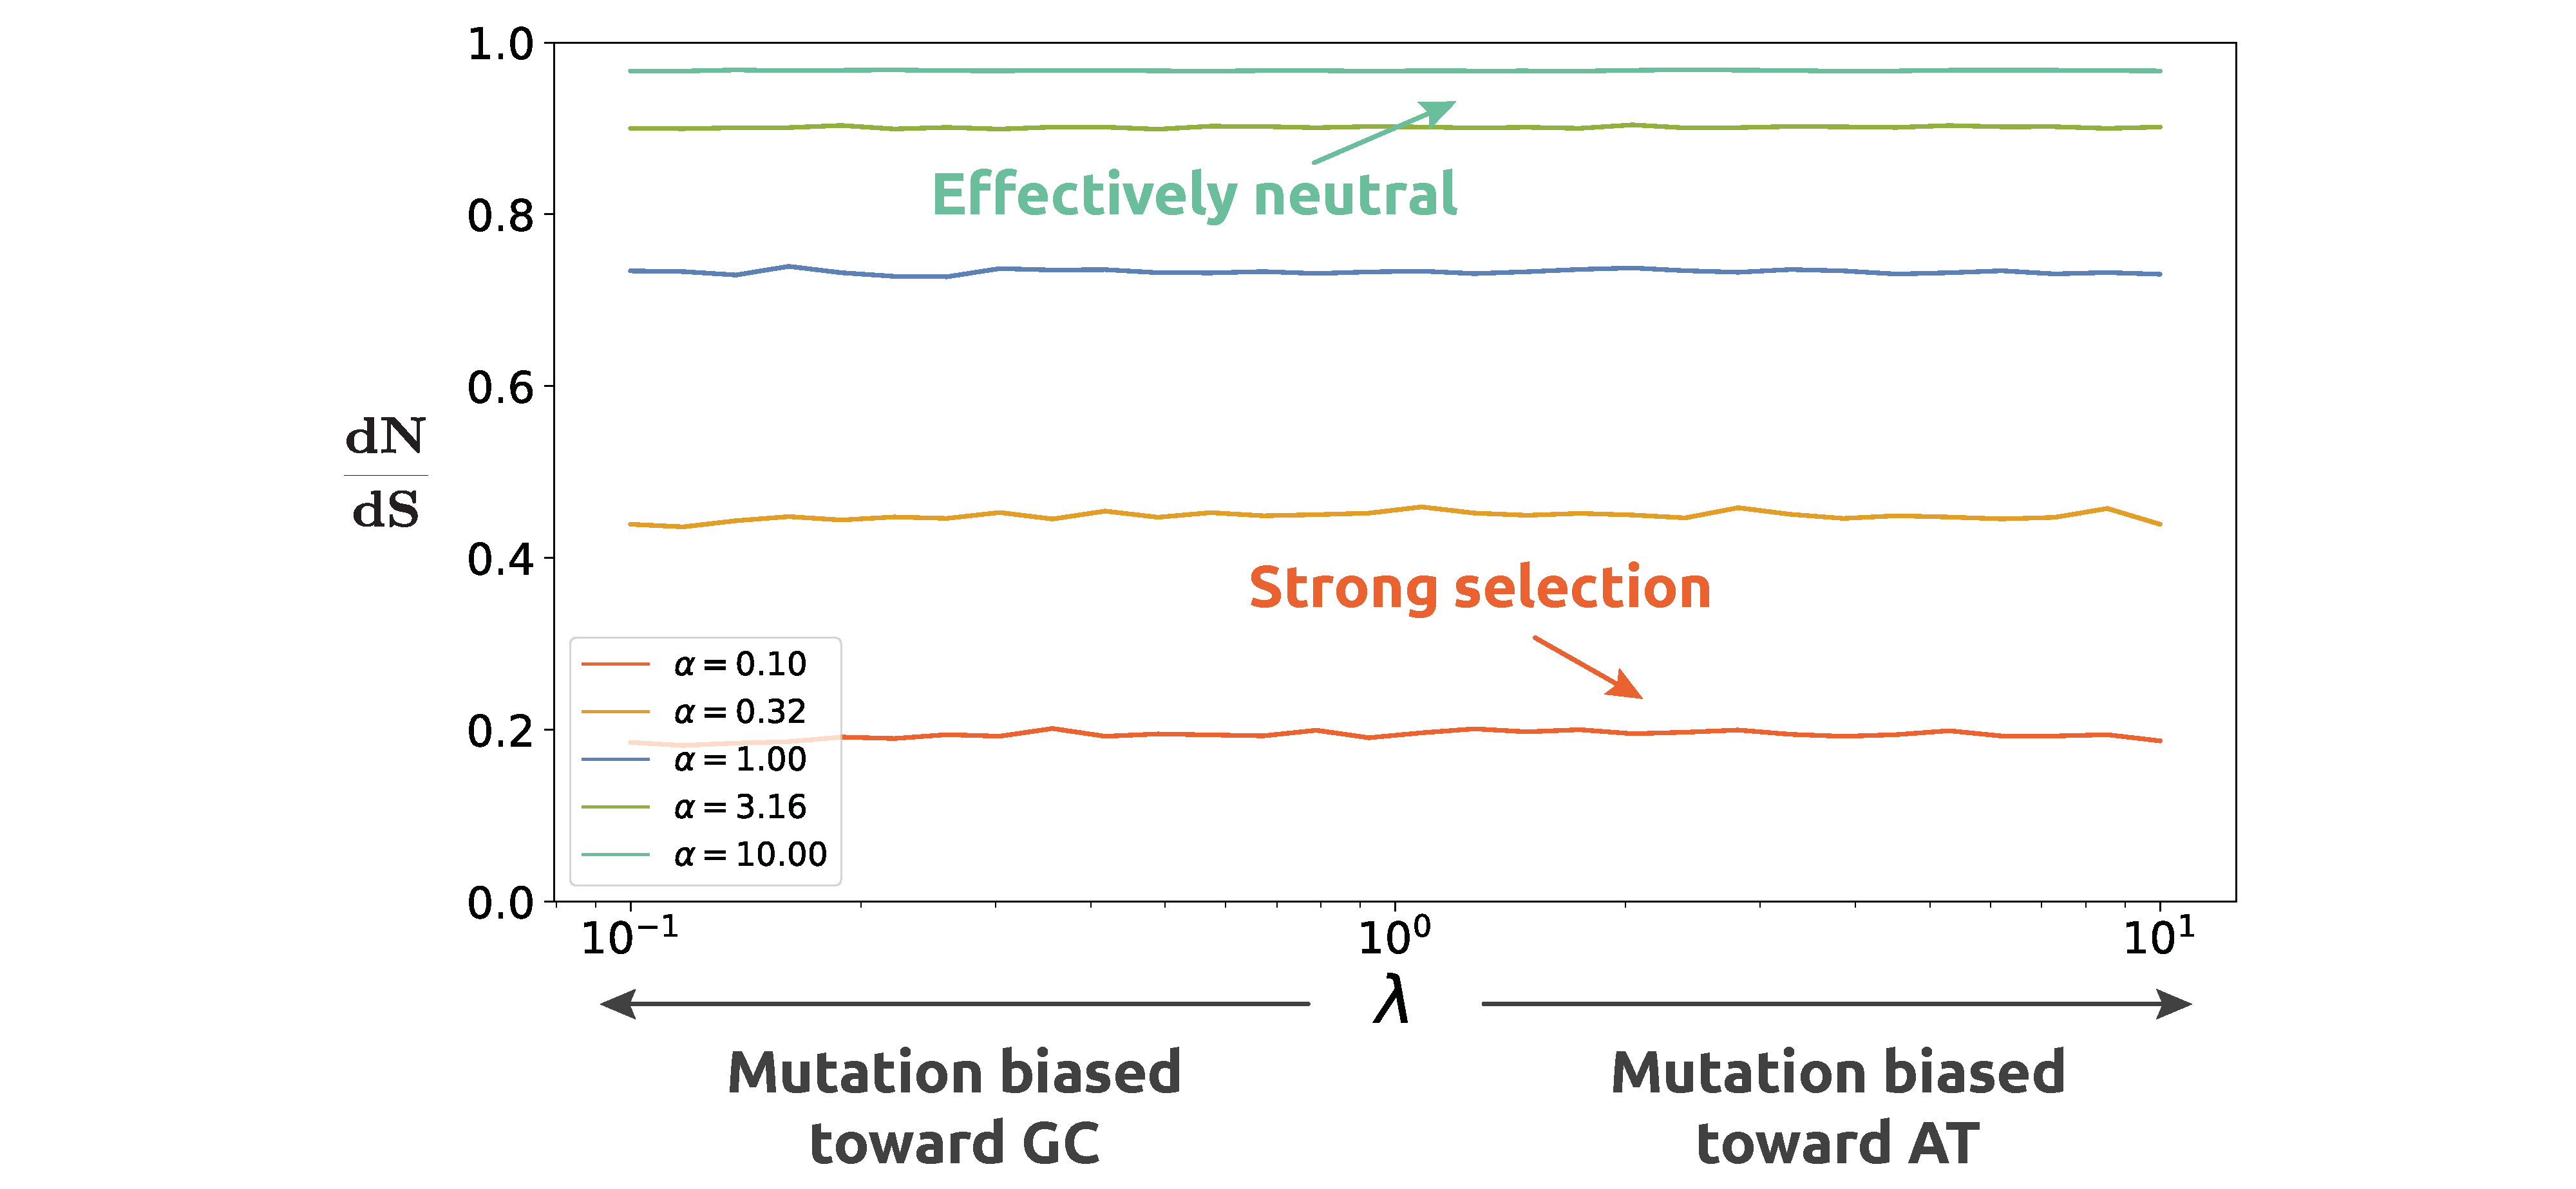
\includegraphics[width=\linewidth, page=1]{omega}
    \end{minipage}
    \llap{\raisebox{-1.0cm}{\scriptsize A\hspace{0.35cm}}}\hfill
    \begin{minipage}{0.32\linewidth}
        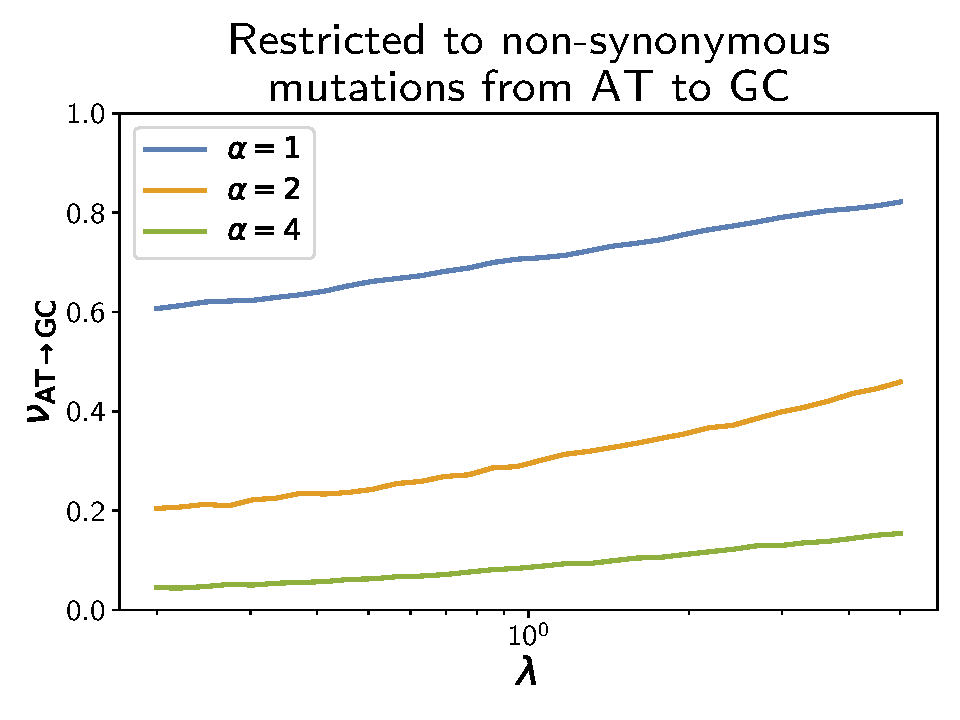
\includegraphics[width=\linewidth, page=1]{omega_WS}
    \end{minipage}
    \llap{\raisebox{-1.0cm}{\scriptsize B\hspace{0.35cm}}}\hfill
    \begin{minipage}{0.32\linewidth}
        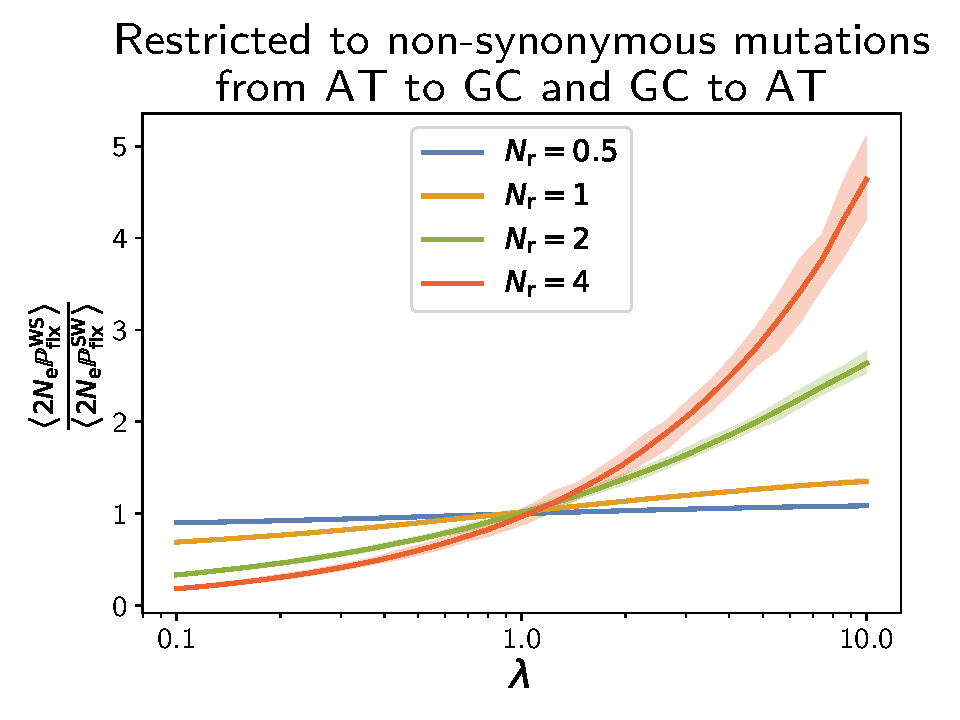
\includegraphics[width=\linewidth, page=1]{omega_WS_over_SW}
    \end{minipage}
    \llap{\raisebox{-1.0cm}{\scriptsize C\hspace{0.35cm}}}\hfill
    \caption[Mean scaled fixation probability as a function of the parameters]{
    Mean scaled fixation probability ($\avgpfix$) in vertical axis as a function of mutational bias ($\lambda$) in the horizontal axis, for different stringency of selection ($\alpha$) in coloured solid lines.
    In panel A, expectedly, $\avgpfix$ decrease with increased strength of selection (i.e.~with decreasing $\alpha$).
    However, $\avgpfix$ is relatively unaffected by the mutational bias ($\lambda$).
    In panel B, $\avgpfix$ is restricted to mutations from weak nucleotides (AT) to strong nucleotides (GC), called $\avgpfix_{\ATtoGC}$, represented in the vertical axis.
    A mutational process biased towards AT leads to an increased fixation probability toward GG, in the opposite direction.
    In panel C, $\avgpfix_{\ATtoGC}$ is divided by the fixation probabilities in the opposing direction $\avgpfix_{\GCtoAT}$, represented in the vertical axis and increasing monotonously with $\lambda$.
    Altogether, mutational bias is balanced by selection in the opposite direction, where this effect increases with the stringency of selection.
    }
    \label{fig:mut-bias-omega-WS}
\end{figure}

\subsection{Parameter inference on simulated data}
\label{subsec:parameter-inference-on-simulated-data}

From an alignment of protein-coding \acrshort{DNA} sequences, without knowing the specific history of substitutions, can one estimate the mutational bias ($\lambda$) and the mean scaled fixation probability ($\avgpfix$)?
In other words, can we tease apart mutation and selection?

To address this question, here we consider two codon models for inference, differing only by their parametrization of the codon matrix $\Submatrix$.
Both are homogeneous along the sequence (i.e.~not site-specific).
The first is based on \citet{Muse1994} formalism and uses a scalar $\omega$ parameter, while the second is based on a tensor representation of $\omega$.

\begin{figure}[htbp]
    \centering
    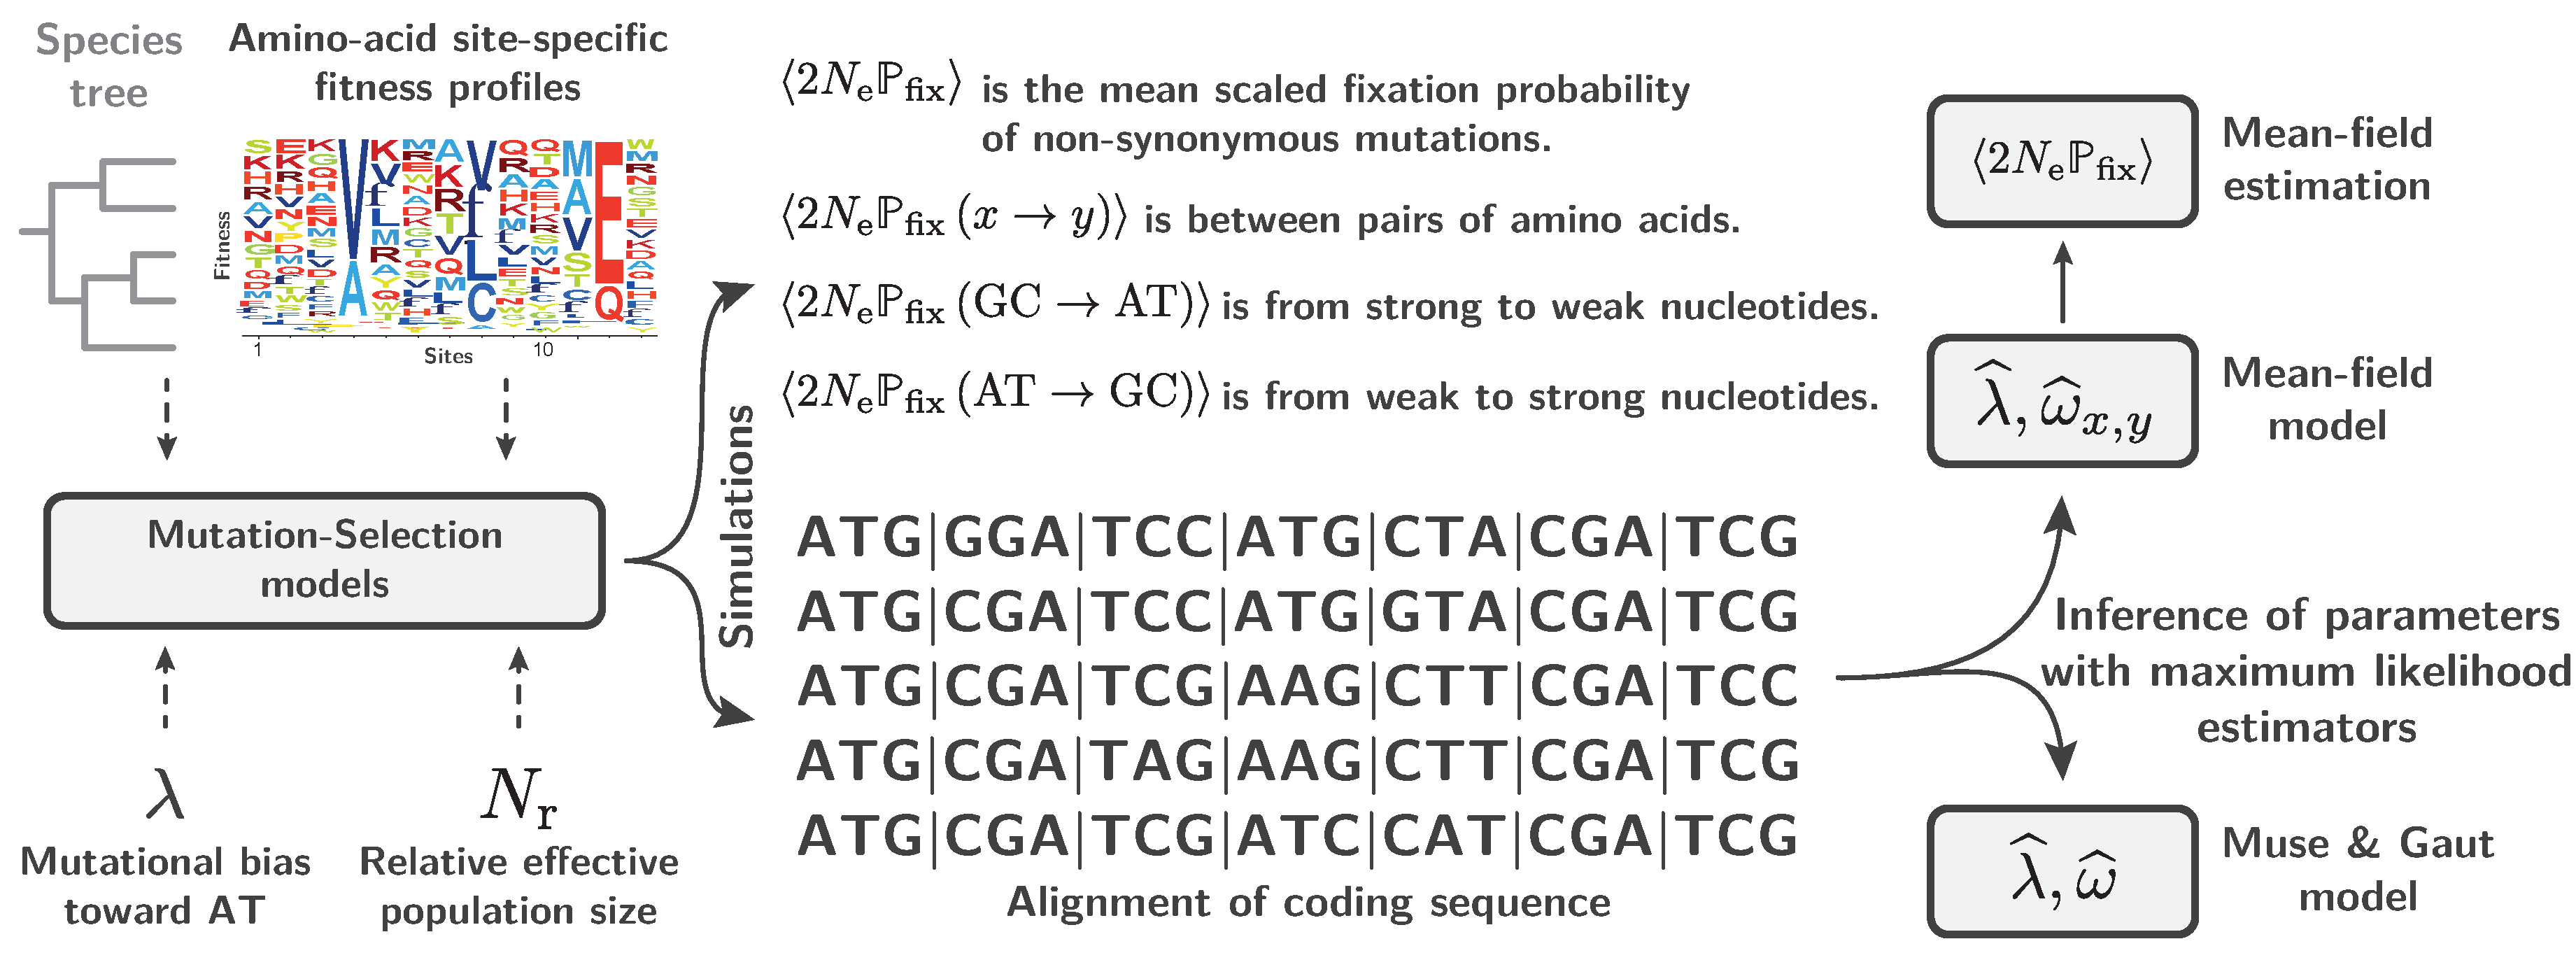
\includegraphics[width=\textwidth, page=1] {pipeline}
    \caption[Inferred value compared to known value]{
    Inferred value ($\widehat{\lambda}$, $\widehat{\avgpfix}$) compared to underlying value ($\lambda$, $\avgpfix$) of the simulation.
    The different parameterization of the inference model can result in different estimates of mutational bias ($\widehat{\lambda}$) and mean scaled fixation probability ($\widehat{\avgpfix}$).
    The main goal is to derive model of inference that can reliably estimate these parameters.
    Two models of inference are proposed, the first is based on Muse \& Gaut formalism, and the second based on a tensor of mean scaled fixation probabilities.}
    \label{fig:mut-bias-pipeline}
\end{figure}

\subsubsection{\texorpdfstring{$\omega$}{ω} as a scalar: the Muse \& Gaut formalism}
This model is defined in terms of a generalized time-reversible nucleotide rate matrix $\Mutmatrix$ and a scalar parameter $\omega$.
The matrix $\Mutmatrix$ is a function of the nucleotide frequencies $\Mutequi$ and the symmetric exchangeability rates $\Exchan$~\citep{Tavare1986}:
\begin{equation}
    \mutmatrix_{a, b} = \exchan_{a,b}\mutequi_b
\end{equation}
At the level of codons, the substitution rate between the source ($\ci$) and target codon ($\cj$) depends on the underlying nucleotide change between ($\nucitoj$) and whether or not the change is non-synonymous.
Altogether, the substitution rates between codons $\submatrix_{\itoj}$, formalized by \citet{Muse1994} are a function of the mutation matrix $\Mutmatrix(\Mutequi, \Exchan)$, a single parameter of selective strength $\omega$, and the genetic code as:
\begin{equation}
    \begin{dcases}
        \submatrix_{\itoj} & = 0 \text{ if codons $\ci$ and $\cj$ are more than one mutation away,} \\
        \submatrix_{\itoj} & = \mutmatrix_{\nucitoj} \text{ if codons $\ci$ and $\cj$ are synonymous,} \\
        \submatrix_{\itoj} & = \omega \mutmatrix_{\nucitoj} \text{ if codons $\ci$ and $\cj$ are non-synonymous}.
    \end{dcases}
    \label{eq:codon-muse-gaut}
\end{equation}

The model can be fitted by maximum likelihood.
Then, from the estimate of $\widehat{\Mutmatrix}$, one can derive a nucleotide bias toward AT as:
\begin{equation}
    \widehat{\lambda}_{\text{MG}} = (\widehat{\mutequi_A} +\widehat{\mutequi_T}) /(\widehat{\mutequi_G} +\widehat{\mutequi_C}).\label{eq:lambda-R}
\end{equation}
As for the mean strength of selection $\widehat{\avgpfix}_{\text{MG}}$, a direct estimate is given by $\widehat{\omega}$.

As shown in the left panel of figure~\ref{fig:mut-bias-inference}, estimate of the mutational bias is halfway between the nucleotide bias observed in the alignment and the true mutational bias used during the simulation.
Thus, the MG model cannot reliably infer the mutational bias.
On the other hand, $\widehat{\omega}$ is close to the underlying mean scaled fixation probability $\avgpfix$ computed during the simulation, with a precision of 98.2\% (not shown).
Thus, the failure to correctly estimate the mutation process does not seem to have a strong impact on the inference of selection, at least in the present case.

\subsubsection{\texorpdfstring{$\omega$}{ω} as a tensor: mean-field derivation}

We would like to derive a codon model that would be more accurate than the Muse \& Gaut model, but that would still be site-homogeneous.
However, the true process is site-specific.
The link between the two can be formalized by projecting the site-specific processes onto a gene-wise process, using what can be seen as a mean-field approximation.
The gene-wise process obtained by this procedure is expressed in terms of mutation rates and mean scaled fixation probabilities.
Finally, the mean scaled fixation probabilities can be identified with the $\omega$-tensor.

Specifically, at each site, the true codon process is:
\begin{equation}
    \begin{dcases}
        \submatrix_{\itoj}\siteexp & = 0 \text{ if codons $\ci$ and $\cj$ are more than one mutation away,} \\
        \submatrix_{\itoj}\siteexp & = \mutmatrix_{\nucitoj} \text{ if codons $\ci$ and $\cj$ are synonymous,} \\
        \submatrix_{\itoj}\siteexp & = \mutmatrix_{\nucitoj} \Pfix\siteexp(\itoj) \text{ if codons $\ci$ and $\cj$ are non-synonymous}.
    \end{dcases}
    \label{eq:codon-site-processs}
\end{equation}
Where $\Pfix\siteexp(\itoj)$ is the scaled fixation probability of codon $\cj$ against codon $\ci$, at site $\site$.
At equilibrium of the process, averaging over sites gives the mean-field gene-level process:
\begin{equation}
    \begin{dcases}
        \left\langle \submatrix_{\itoj} \right\rangle & = 0 \text{ if codons $\ci$ and $\cj$ are more than one mutation away,} \\
        \left\langle \submatrix_{\itoj} \right\rangle & = \mutmatrix_{\nucitoj} \text{ if codons $\ci$ and $\cj$ are synonymous,} \\
        \left\langle \submatrix_{\itoj} \right\rangle & = \mutmatrix_{\nucitoj} \left\langle \Pfix (\itoj) \right\rangle \text{ if codons $\ci$ and $\cj$ are non-synonymous}.
    \end{dcases}
    \label{eq:codon-avg-process}
\end{equation}
However, because selection between codons reduces to selection between pairs of amino-acids, $\left\langle \Pfix (\itoj) \right\rangle$ only depends on the amino-acids encoded by $\ci$ and $\cj$ (section~\ref{subsec:mean-field-derivation} in methods).
Thus, by identification, the inference model should be parameterized by a set of $\omega$ values for all pairs of amino acids, denoted $\omega_{\aaSource, \aaTarget}$.
For $20$ amino acids, the total number of pairs of amino acids is $190$, hence $380$ parameters by counting in both directions.
However, because of the structure of the genetic code, they are $75$ pairs that are one nucleotide away, since some amino acids are not directly accessible through a single non-synonymous mutation.
As a result, the number of parameters necessary to determine all non-zero entries of the tenser ($\omega_{\aaSource, \aaTarget}$) in both directions is $150$.
Finally, under the assumption of a reversible process, the number of parameters can be reduced to $75$ symmetric exchangeabilities ($\AAexchan_{\aaSource, \aaTarget}$) and $20$ stationary effects ($\AAequi_{\aaSource}$):
\begin{equation}
    \omega_{\aaSource, \aaTarget} = \AAequi_{\aaTarget} \AAexchan_{\aaSource, \aaTarget}\text{, where } \AAexchan_{\aaSource, \aaTarget} = \AAexchan_{\aaTarget, \aaSource}.\label{eq:omega-reversible}
\end{equation}

Altogether, the substitution rates between codons $\submatrix_{\itoj}$ are defined as:
\begin{equation}
    \begin{dcases}
        \submatrix_{\itoj} & = 0 \text{ if codons $\ci$ and $\cj$ are non neighbors}, \\
        \submatrix_{\itoj} & = \mutmatrix_{\nucitoj} \text{ if codons $\ci$ and $\cj$ are synonymous,}, \\
        \submatrix_{\itoj} & = \mutmatrix_{\nucitoj} \omega_{\aai, \aaj} \text{ if codons $\ci$ and $\cj$ are non-synonymous},
    \end{dcases}
    \label{eq:codon-mean-field}
\end{equation}
where $\aai$ is the amino acid encoded by codon $\ci$ and $\omega_{\aaSource, \aaTarget}$ is given by equation~\ref{eq:omega-reversible}.

This mean-field (MF) model is fitted by maximum likelihood, giving an estimate for its parameters, $\widehat{\Mutmatrix}$, $\widehat{\AAExchan}$ and $\widehat{\AAEqui}$.
Then, from the estimate of the GTR nucleotide matrix ($\widehat{\Mutmatrix}$), a mutation bias $\widehat{\lambda}_{\text{MF}}$ can be estimated as previously (equation~\ref{eq:lambda-R} above).

As shown in the right panel of figure~\ref{fig:mut-bias-inference}, $\widehat{\lambda}_{\text{MF}}$ under the MF model provides an accurate estimate of the true mutational.
In other words, the MF model can tease out the observed $\atgc$ bias of the alignment and the underlying mutational bias.

The mean scaled fixation probability of non-synonymous mutations $\widehat{\avgpfix}_{\text{MF}}$ can also be computed.
It is now a compound parameter, expressed as a function of $\widehat{\Mutmatrix}$, $\widehat{\AAExchan}$ and $\widehat{\AAEqui}$ (see section~\ref{sec:mut-bias-mean-field-omega}).
Under this model, $\widehat{\avgpfix}_{\text{MF}}$ is close to the true mean scaled fixation probability $\avgpfix$ computed during the simulation, with a precision of 97.0\% (not shown).

\begin{figure}[htbp]
    \centering
    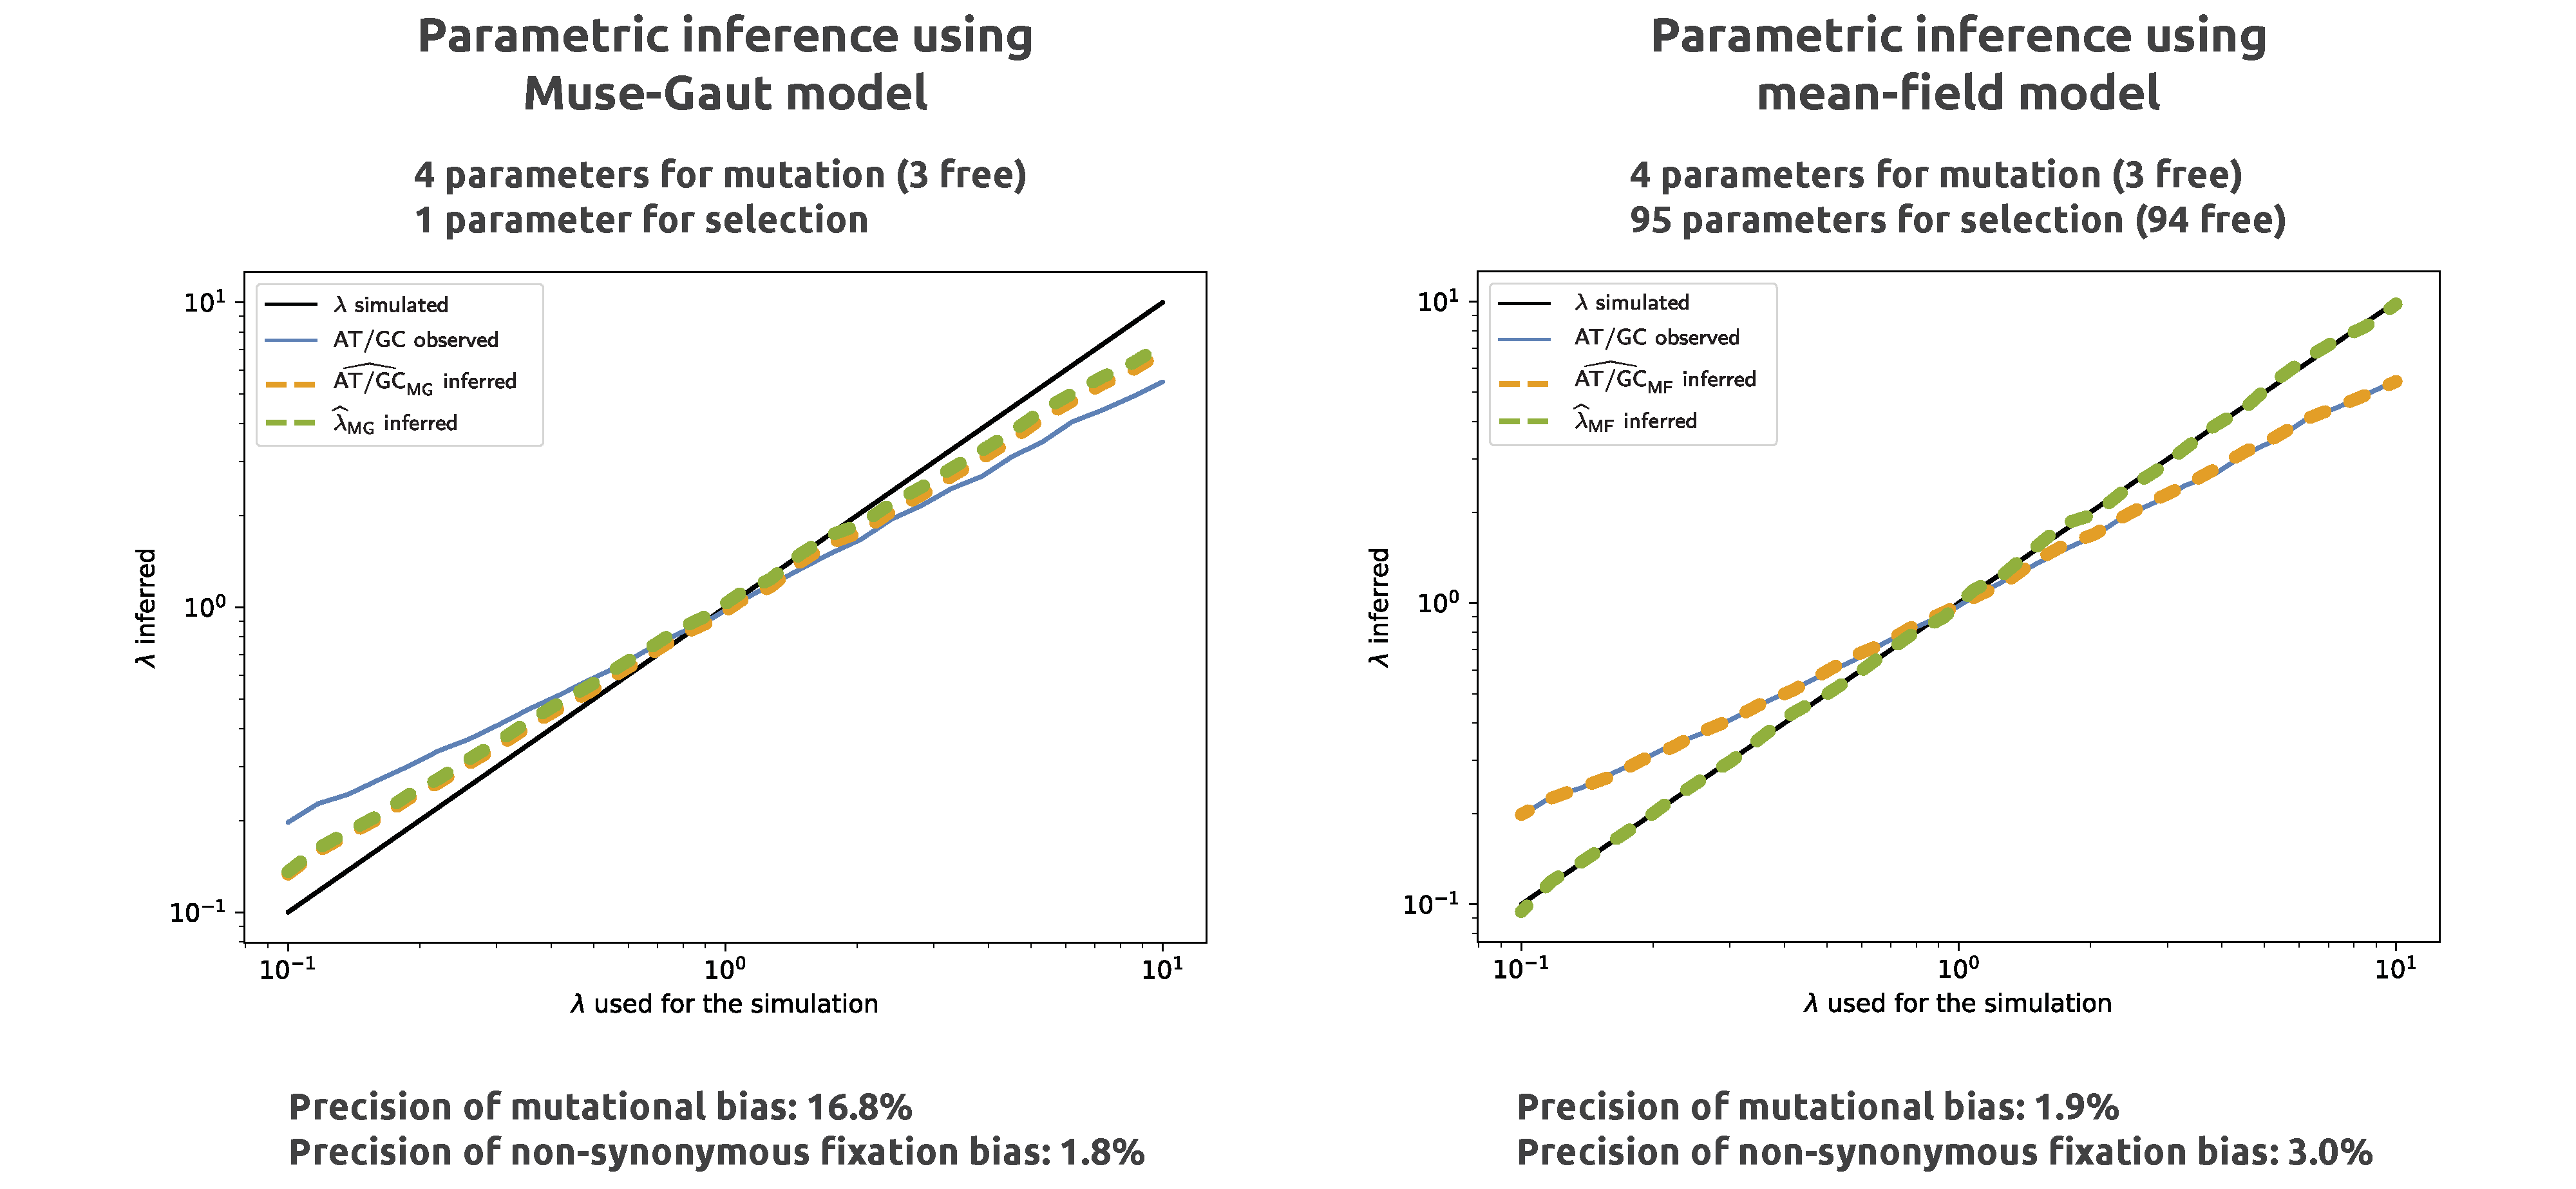
\includegraphics[width=\textwidth] {Simulation-vs-Inference}
    \caption[Estimation of mutational bias]{
    Different proxies of estimated mutational bias in the vertical axis are represented as a function of the underlying mutational bias ($\lambda$) of the simulation in the horizontal axis.
    Mutational bias can be estimated directly from the observed nucleotide frequencies in the alignment ($\atgc$ in blue solid line), similarly to figure~\ref{fig:mut-bias-AT-GC-obs}, which is skewed by selection and always less extreme than the underlying mutational bias.
    The robustness of mutational bias estimation of two different inference models are shown.
    Selection is modelled as a single $\omega$ parameter in the Muse \& Gaut formalism (MG) in the left panel, while selection is modelled as a tensor of $\omega$ parameters in different directions using a mean-field (MF) approximation in the right panel.
    In both panels, the true value of the mutational bias is represented in black solid line.
    The estimated mutational bias $\widehat{\lambda}_{\text{MG}}$ (in yellow dotted line) in the MG formalism is between the true value and the observed $\atgc$.
    Conversely, estimated mutational bias $\widehat{\lambda}_{\text{MG}}$ (in yellow dotted line) in the MF approximation equal to the underlying value.
    Moreover, the expected $\widehat{\atgc}$ from the parameter of the model fits the observed value in the MF approximation, while being skewed in the MG formalism.
    Altogether, the MF approximation can tease apart mutation and selection, while the MG formalism has to reach a compromise between observed $\atgc$ and underlying mutational bias.
    }
    \label{fig:mut-bias-inference}
\end{figure}

\subsection{Estimation of empirical sequence data}
\label{subsec:estimation-of-empirical-sequence-data}

The two alternative models of inference just considered, namely the classical Muse \& Gaut (MG) and the mean-field (MF) codon models, were then applied to empirical protein-coding sequence alignments.
Two examples were analysed: the nucleoprotein in \textit{Influenza Virus} assembled in \citet{Bloom2017}, and the $\beta$-lactamase in \textit{bacteria} gathered in \citet{Bloom2014}, as shown in table~\ref{tab:mut-bias-estimation}.

The nucleoprotein alignment of 498 amino acids is available for 180 virus strains (as human host), and is globally biased toward AT.
Similarly to what was observed in the simulation experiments presented above, the mutational bias estimates under the two codon models are greater than the observed nucleotide bias (i.e.~$1 < \atgc < \widehat{\lambda}$).
This effect is, as previously, probably due to selection at the level of amino acids, partially opposing the mutational bias.
More importantly, the mutational bias estimated by the MF model is more extreme than the MG estimate (i.e.~$1 < \widehat{\lambda}_{\text{MG}} < \widehat{\lambda}_{\text{MF}}$).
This example behaves identically to the observations made with simulated alignments, where, compared to MG, the MF model estimates a stronger mutational bias, which was also closer to the real value.
Thus, a reasonable interpretation is that MG is also underestimating the underlying mutational bias in the present case, and that the estimate of the MF model is more accurate.

Concerning selection, the estimated mean scaled fixation probability of non-synonymous mutations, denoted $\widehat{\avgpfix}$, is similarly estimated in the MG and MF models ($\widehat{\avgpfix}_{\text{MG}} \simeq \widehat{\avgpfix}_{\text{MF}}$).
Additionally, in the MF model, $\widehat{\avgpfix}_{\text{MF}}$ can be restricted to mutations from weak nucleotides (AT) to strong (GC), or vice versa (see section~\ref{sec:mut-bias-mean-field-omega}).
We observe that under a mutational bias favouring AT (i.e.~$\lambda > 1$), the mean fixation probability of non-synonymous mutations is higher toward GC than toward AT (i.e.~$\widehat{\avgpfix}_{MF,\ATtoGC} > \widehat{\avgpfix}_{MF,\GCtoAT}$), as expected if the mutational bias is toward AT.

Reciprocally, for the $\beta$-lactamase, the alignment of 263 amino acids available for 85 species is globally biased toward GC.
Expectedly, the mean-field estimate is even more strongly biased toward GC (i.e.~$\widehat{\lambda}_{\text{MF}} < \atgc < 1$).
Curiously, the MG model estimates a weaker underlying mutational bias than the observed bias (i.e.~$ \atgc < \widehat{\lambda}_{\text{MG}} < 1$).
Concerning selection, we observe that the fixation probability of non-synonymous mutations is higher on average toward AT than toward GC (i.e.~$\widehat{\avgpfix}_{MF,\GCtoAT} > \widehat{\avgpfix}_{MF,\ATtoGC}$), again, as expected under a GC-biased mutation process.

Altogether, the results obtained on empirical data are globally in agreement with the observations gathered from the simulation experiments, namely that the presence of a mutational bias results in a selection differential, taking the form of a slightly higher mean fixation probability of non-synonymous mutations opposing the mutational bias.
Our MF model detects this effect and simultaneously estimates more extreme (and probably more accurate) mutational biases compared to the MG model.

\begin{table}[htbp]
    \centering
    \noindent\adjustbox{max width=\textwidth}{%
    \begin{tabu}{|c||c|c|}
        \hline
        & \textbf{Nucleoprotein} & \textbf{Lactamase} \\
        \hline \textbf{Number of sites} & 498 & 263 \\
        \hline \textbf{Number of taxa} & 180 & 85 \\
        \hline \textbf{$\atgc$ of the alignment} & 1.15 & 0.79 \\
        \hline \textbf{$\atgc$ at first coding position} & 1.06 & 0.58 \\
        \hline \textbf{$\atgc$ at second coding position} & 1.22 & 1.18 \\
        \hline \textbf{$\atgc$ at third coding position} & 1.19 & 0.71 \\
        \hline \textbf{Muse \& Gaut mutational bias ($\widehat{\lambda}_{\text{MG}}$)} & 1.39 & 0.85 \\
        \hline \textbf{Mean-field mutational bias ($\widehat{\lambda}_{\text{MF}}$)} & 1.64 & 0.68 \\
        \hline \textbf{Site diversity} & 1.10 & 1.37 \\
        \hline \textbf{Muse \& Gaut scaled fixation probability ($\widehat{\avgpfix}_{\text{MG}}$)} & 0.085 & 0.29 \\
        \hline \textbf{Mean-field scaled fixation probability ($\widehat{\avgpfix}_{\text{MF}}$)} & 0.086 & 0.30 \\
        \hline \textbf{Mean-field scaled fixation probability} & \multirow{2}{*}{0.14} & \multirow{2}{*}{0.31} \\
        \textbf{from AT to GC ($\widehat{\avgpfix}_{\text{MF},\ATtoGC}$)} & & \\
        \hline \textbf{Mean-field scaled fixation probability} & \multirow{2}{*}{0.10} & \multirow{2}{*}{0.44} \\
        \textbf{from GC to AT ($\widehat{\avgpfix}_{\text{MF},\GCtoAT}$)} & & \\
        \hline \textbf{$\widehat{\avgpfix}_{\text{MF},\ATtoGC} / \widehat{\avgpfix}_{\text{MF},\GCtoAT}$ } & 1.36 & 0.71 \\
        \hline
    \end{tabu}}
    \caption[Estimated parameters]{
    Estimated parameters of mutational bias ($\widehat{\lambda}$) from two models of inference, namely classical Muse \& Gaut (MG) and mean-field (MF).
    These models are applied to two distinct datasets of protein-coding DNA alignment, nucleoprotein in the left column and $\beta$-lactamase in the right column.
    By taking into account selection in multiple direction, MG models estimates stronger mutational bias than the MG model.
    For the MG model the mean scaled fixation probability of non-synonymous mutations ($\widehat{\avgpfix}_{MF}$) can be obtained either from weak (AT) to strong nucleotides (GC), or vice versa.
    The fixation probability of non-synonymous mutations is opposed to the underlying mutational bias, such that a skewed mutational process results in a skewed selection, justifying that they must be articulated together.
    }
    \label{tab:mut-bias-estimation}
\end{table}


\section{Discussion}\label{sec:discussion}

In protein-coding DNA sequences, the nucleic composition results from a subtle interplay between mutation at the nucleic level and selection at the protein level.
As a result, the observed nucleotide bias in the alignment is different from the underlying mutational bias.

However, current parametric codon models are inherently misspecified and, for that reason, are unable to tease apart these opposing effects of mutation and selection correctly.
As a result, they don’t estimate the mutational process reliably.

In this work we seek to find the simplest parametric codon model able to correctly tease apart mutation rates on one hand, and net mean fixation probabilities on the other hand, and this, without having to explicitly model the underlying fitness landscape.
In order to derive a codon model along those lines, our strategy is to first assume an underlying microscopic model of sequence evolution (here, a mutation-selection model based on a site-specific, time-independent fitness landscape).
Then, we derive the gene-wise mean fixation probabilities between all pairs of codons, implied by the underlying microscopic process.
Finally, we observe that this mean-field process should in fact invoke as many distinct $\omega$ parameters as there are pairs of amino acids that are nearest neighbours in the genetic code.
There are reversibility conditions, reducing the dimensionality and allowing for a GTR-like parameterization of this tensor ($95$ parameters for selection).

Inferring parameters on simulated alignments, we show that the model derived using this mean-field argument correctly estimates the underlying mutational bias and selective pressure.
Applied to empirical alignments, we also observed that there is a selection differential opposing the mutational bias.

This work first points to a fundamental property of natural genetic sequences, namely that they are not optimized but are the result of an equilibrium between forces.
In the specific case highlighted in this work, mutational bias at the nucleotide-level results in suboptimal amino-acid being overrepresented in the sequence.
This was pointed out previous~\citep{Singer2000}, although never directly formalized in the context of a phylogenetic codon model.

One important consequence of this tradeoff between mutation and selection at equilibrium is that the observed higher mean fixation probability toward GC is mimicking the effect of biased gene conversion toward GC (gBGC), although unlike gBGC, the phenomenon described here corresponds to a genuine selective effect.
Although we did not explore the consequences of this at the level of intra-specific polymorphism, the selection differential uncovered here also implies that the distribution of fitness effects is not the same in the two directions, either toward AT or toward GC.
Specifically, in the presence of an AT-biased mutation process, the non-synonymous GC polymorphisms are expected to segregate at higher frequencies, compared to non-synonymous AT polymorphisms.

These observations have some practical implications: for instance, experiments observing a fixation (or segregation) bias toward GC at the non-synonymous level must also rule out that this fixation bias is not the simple consequence of the mutation-selection balance.
More generally, our observations and modelling principles offer a useful preliminary basis to better understand how mutation and selection will work together with biased gene conversion (gBGC), and therefore will help better understand of how gBGC will impact both nucleotide composition and the $\dnds$.
It worth mentioning that in our result, we focused on the fixation probability from AT to GC ($\avgpfix_{\ATtoGC}$) because of the relationship to gBGC.
However, in practice, the same analysis and methods can be applied to any subset of nucleotides or codons.

Our mean-field parametric model uses gene-level parameters (in the form of a tensor) that is meant to capture the mean scaled fixation probabilities.
This derivation, and its validation on simulated data, shows that, even though the underlying selective landscape is site-specific, a gene-level approximation can nonetheless accurately disentangles mutation and selection.
As a result, this study demonstrates that phenomenological models derived out of mechanistic models are more compact (i.e.~not site-specific), and in certain cases are sufficient to extract the relevant parameters.

The methodology proposed here for deriving inference models consists in proceeding in two steps, first assuming an underlying mechanistic model of sequence evolution, parameterized by variables that are derived from first principles (fitness landscape, mutations rates, $\hdots$).
Subsequently, the phenomenological inference model is obtained by matching its parameters (here, the entries of the $\omega$ tensor) with the aggregate parameters derived from the application of the mean-field procedure to the mechanistic model.
Altogether, we believe that the approach used here could be applied more generally: inference model can be phenomenological in practice, but should nonetheless be derived from an underlying mechanistic model, so as to correctly formalize the interplay between, mutation, selection, drift and other evolutionary forces.

Finally, this work is still preliminary, and the mean-field model should be tested against a more diverse range of empirical data, in terms of phylogenetic depth, strength of selection, codon usage bias to assert for the validity of our empirical results.
Also, the empirical fit to the data between the models (e.g.~using AIC) should be more carefully examined.
Indeed, by setting $\AAEqui = \vecOne$ and $\AAExchan = \omega \times \vecOne$ in our mean-field models, we retrieve the nested Muse \& Gaut model, hence both models are directly comparable.
In addition, several other codon models~\citep{Rodrigue2008a,KosakovskyPond2020} should be included in a broader comparison of the accuracy of the estimation of the underlying mutational bias and strength of selection on protein-coding DNA sequences.


\section{Materials \& Methods}

\subsection{Simulation model}
\label{sec:mut-bias-simu}
We seek to simulate the evolution of protein-coding sequences along a specie tree.
Starting with one sequence at the root of the tree, the sequences evolve independently along the different branches of the tree by point substitutions, until they reach the leaves.
At the end of the simulation, we get one sequence for each leaf of the tree, meaning one sequence per species.
The substitution is modelled using the origination-fixation approximation, i.e.~substitution rates are the product of the mutation rate at the nucleotide level, and fixation probabilities, based on selection at the amino-acid level.

The mutation process is assumed homogeneous across sites.
On the other hand, selection is assumed to be varying along the sequence.
During the simulation, given the current sequence, the substitution rates toward all possible mutants (one nucleotide change) are computed and the next substitution event is drawn randomly based on Gillespie’s algorithm ~\citep{Gillespie1977}.

\subsection{Mutational bias at the nucleotide level}
\label{sec:mut-bias-mut-matrix}
The mutation rate between nucleotides is always proportional to $\mu$.
Moreover, mutations from any nucleotide to another weak nucleotide is increased by the factor $\lambda$ compared with mutations to another strong nucleotide.
The mutation rate matrix is thus:
\begin{equation}
    \label{nucMatrix}
    \Mutmatrix =
    \begin{blockarray}{ccccc}
        & A & C & G & T \\
        \begin{block}{c(cccc)}
            A & {-\mu(2 + \lambda)} & {\mu} & {\mu} & {\mu \lambda} \\
            C & {\mu \lambda} & {-\mu(1 + 2\lambda)} & {\mu} & {\mu \lambda} \\
            G & {\mu \lambda} & {\mu} & {-\mu(1 + 2\lambda)} & {\mu \lambda} \\
            T & {\mu \lambda} & {\mu} & {\mu} & {-\mu(2 + \lambda)} \\
        \end{block}
    \end{blockarray}
\end{equation}
Which has the following stationary distribution:
\begin{align}
    \Mutequi \Mutmatrix & = \vecOne, \\
    \iff \Mutequi & = \left( \dfrac{\lambda}{2+2\lambda}, \dfrac{1}{2+2\lambda}, \dfrac{1}{2+2\lambda}, \dfrac{\lambda}{2+2\lambda} \right).
    \label{nucStationarity}
\end{align}
The process is reversible and fulfills the detailed balance condition, i.e.~for any pair of distinct nucleotides:
\begin{equation}
    \mutequi_a \mutmatrix_{a, b} =\mutequi_b \mutmatrix_{b, a}.
    \label{nucMutBalance}
\end{equation}
As a result, the ratio of weak over strong nucleotide frequencies at stationarity is equal to $\lambda$:
\begin{align}
    \label{lambda}
    \dfrac{ \mutequi_A + \mutequi_T }{ \mutequi_C + \mutequi_G }
    & = \dfrac{ \lambda ( 2 + 2 \lambda)^{-1} + \lambda ( 2 + 2 \lambda)^{-1}}{ ( 2 + 2 \lambda)^{-1} + ( 2 + 2 \lambda)^{-1}}, \ \text{from eq.~\ref{nucStationarity},}\\
    & = \lambda.
\end{align}

\subsection{Selection at the amino-acid level}
\label{sec:mut-bias-aa-selection}

The substitution rate is considered null between any two codons differing by more than one nucleotide.
Otherwise, the mutation rate between a pair of codons is given by the mutation rate of the underlying single nucleotide change.
Selection is modelled at the amino-acid level, i.e.~we assume that all codons encoding for one particular amino acid are selectively neutral.

To take into account the heterogeneity of selection between different sites of the protein, we assume that each site $\site$ of the sequence is independently evolving under a site-specific fitness landscape, characterized by a 20-dimensional frequency vector of scaled (Wrightian) fitness parameters $\Profile\siteexp = \{ \profile\siteexp_{\aminoacid},\ 1 \leq \aminoacid \leq 20 \}$.
The (Wrigthian) fitness vectors across sites are drawn IID from a uniform Dirichlet distribution prior to the simulation over the tree:
\begin{equation}
    \Profile\siteexp \sim \text{Dirichlet} (\alpha, \hdots, \alpha), \Setsite,
\end{equation}
The malthusian fitness (or log-fitness) of amino acid $\aminoacid$, denoted $\scaledfit\siteexp_{\aminoacid}$, is accordingly:
\begin{equation}
    \scaledfit\siteexp_{\aminoacid} = \ln \left( \profile\siteexp_{\aminoacid} \right),\ \Setsite, \ \SetAa
\end{equation}
At site $\site$, the substitution rate between non-synonymous codons $\ci$ and $\cj$ is given by the product of the mutation rate and the probability of fixation:
\begin{equation}
    \submatrix_{\itoj}\siteexp = \mutmatrix_{\nucitoj} \dfrac{\Fitj\siteexp - \Fiti\siteexp}{1 - \e^{\Fiti\siteexp - \Fitj\siteexp} } \label{eq:codonsubrates}
\end{equation}
where $\aai$ denotes the amino-acid encoded by codon $\ci$.
At the root of the tree, for each site $\site$, the sequence is drawn from the stationary distribution of the process specified by $\Subequi\siteexp$, which is given by:
\begin{align}
    \subequi_{\ci}\siteexp & = \mathcal{Z}\siteexp \left[\prod\limits_{k \in \{ 1, 2, 3 \}} \mutequi_{\ci[k]}\right] \e^{\Fiti\siteexp},
    \label{codonStationarity}
\end{align}
where $\ci[k]$ denotes the nucleotide at position $k \in \{ 1, 2, 3 \}$ of codon $\ci$, and $\mathcal{Z}\siteexp $ is the normalizing constant at site $\site$:
\begin{align}
    \mathcal{Z}\siteexp = \left( \sum\limits_{\jSetCodon} \left[\prod\limits_{k \in \{ 1, 2, 3 \}} \mutequi_{\cj[k]}\right] \e^{\Fitj\siteexp} \right)^{-1}
\end{align}
The substitution process is reversible and fulfils detailed balance conditions at each site $\site$ and between each pair of codons ($\ci$, $\cj$):
\begin{align}
    \subequi_{\ci}\siteexp \submatrix_{\itoj}\siteexp = \subequi_{\cj}\siteexp \submatrix_{\cj, \ci}\siteexp
    \label{codonSubBalance}
\end{align}

Of note, by modelling fitness at the amino-acid level, we assume that all codons encoding for one particular amino acid are selectively neutral.
In addition, in this modelling framework, the genetic code is of particular importance since the number of codons encoding for a particular amino acid varies greatly.
As an example, tryptophan is encoded by one codon, while leucine is encoded by 6 codons.
Intuitively, this variation makes the mutation bias more pronounced among codons encoding for the same amino acid, since there are more mutations possible that are selectively neutral (i.e. synonymous).
On the other hand, the mutation bias is more constrained if the amino acid is encoded by few codons.

\subsection{Site and sequence diversity of amino-acids}
\label{subsec:entropy}

For a site $\site$, the diversity $D\siteexp$ (or effective number of amino acids) is computed as the exponential of Shannon's entropy from the frequencies of the different amino-acids $\Freq\siteexp = \{ \freq\siteexp_{\aminoacid},\ \SetAa$, as:
\begin{equation}
    D(\Freq\siteexp) = \exp \left[ - \sum\limits_{\SetAa} \freq\siteexp_{\aminoacid} \ln \left( \freq\siteexp_{\aminoacid} \right) \right]
    \label{eq:diversity-site-specific}
\end{equation}
The diversity is a measure of the sparsity of the amino-acid frequencies, with a value of $1$ corresponding to the minimum diversity (i.e.~with only one amino acid permissible), and a value of $20$ corresponding to maximum diversity, where each amino acid has the same frequency.
The diversity can be first computed for each site and then averaged over all sites as:
\begin{equation}
    \left\langle D(\Freq) \right\rangle = \dfrac{1}{\Nsite}\sum\limits_{\Setsite} D(\Freq\siteexp)
    \label{eq:diversity-site-specific-avg}
\end{equation}
Alternatively, average frequencies of the different amino acids can first be computed over the alignment and then used to compute the global sequence diversity:
\begin{equation}
    \left\langle \Freq \right\rangle = \dfrac{1}{\Nsite}\sum\limits_{\Setsite} \Freq\siteexp
    \label{eq:profile-gene-wise}
\end{equation}
Then the sequence diversity is simply:
\begin{equation}
    D \left(  \left\langle \Freq \right\rangle \right) = \exp \left[ - \sum\limits_{\SetAa} \left\langle \freq \right\rangle_{\aminoacid} \ln \left( \left\langle \freq \right\rangle_{\aminoacid} \right) \right]
    \label{eq:diversity-gene-wise}
\end{equation}

\subsection{Mean scaled fixation probability}
\label{subsec:fixation-bias}
The sequence at time $t$ is denoted $\Seqi(t)$ and the codon present at site $\site$ is denoted $\Seqi_{\site}(t)$.
For a given sequence, the mean scaled fixation probability over mutations away from $\Seqi(t)$ (weighted by their probability of occurrence) is given by the ratio:
\begin{align}
    \avgpfix (t) & = \dfrac{ \sum\limits_{\Setsite} \sum\limits_{\cj \in \NonSynNeighbors \left ( \Seqi_{\site}(t) \right)} Q_{\Seqi_{\site}(t) \to \cj}}{ \sum\limits_{\Setsite} \sum\limits_{\left ( \cj \in \Seqi_{\site}(t) \right)} \mu_{\Seqi_{\site}(t) \to \cj}},
\end{align}
where $\setNonSynNeighbors$ is the set of non-synonymous codons neighbours of codon $\ci$ and $\submatrix_{\itoj}\siteexp$ are defined as in equation~\ref{eq:codonsubrates}.
Averaged over all branches of the tree, the mean scaled fixation probability is :
\begin{align}
    \avgpfix & = \left\langle \avgpfix (t) \right\rangle, \\
    & = \int_{t} \avgpfix (t) \der t,
\end{align}
where the integral is taken over all branches of the tree, while the integrand $\avgpfix (t)$ is a piece-wise function changing after every point substitution event.
The mean scaled fixation probability from weak (AT) to strong (GC) nucleotides, denoted $\avgpfix_{\ATtoGC}$, is obtained similarly by restricting the sums (in the numerator and the denominator) from weak to strong mutations.
A similar computation can be done from strong to weak.

\subsection{Derivation of mean-field model}
\label{subsec:mean-field-derivation}
Assuming an underlying site-specific mutation-selection process at equilibrium, given we know that a mutation is from codon $\ci$, the probability that this mutation is occuring at site $\site$ is:
\begin{align}
    \proba (\site \mid \ci) = \dfrac{ \subequi_{\ci}\siteexp }{\sum\limits_{\Setsite} \subequi_{\ci}\siteexp }
\end{align}
The site-averaged (mean-field) substitution rate from codon $\ci$ to $\cj$ is as result given as:
\begin{align}
    \left\langle \submatrix_{\itoj} \right\rangle = \sum\limits_{\Setsite} \proba (\site \mid \ci) \submatrix_{\itoj}
\end{align}
If codon $\ci$ and codon $\cj$ are synonymous, this equation simplifies to the underlying mutation rate $\mutmatrix_{\nucitoj}$.
Otherwise, if codon $\ci$ and codon $\cj$ are non-synonymous, the mean-field substitution rate is:
\begin{align}
    \left\langle \submatrix_{\itoj} \right\rangle & = \left\langle \mutmatrix_{\nucitoj} \Pfix (\itoj) \right\rangle, \\
    & = \mutmatrix_{\nucitoj} \left\langle \Pfix (\itoj) \right\rangle, \\
    & = \mutmatrix_{\nucitoj} \dfrac{ \sum\limits_{\Setsite} \subequi_{\ci}\siteexp \dfrac{\Fitj\siteexp - \Fiti\siteexp}{1 - \e^{\Fiti\siteexp - \Fitj\siteexp}} }{ \sum\limits_{\Setsite} \subequi_{\ci}\siteexp }, \\
    & = \mutmatrix_{\nucitoj} \dfrac{ \sum\limits_{\Setsite} \mathcal{Z}\siteexp  \dfrac{\Fitj\siteexp - \Fiti\siteexp}{ \e^{-\Fiti\siteexp} - \e^{ - \Fitj\siteexp}} }{  \sum\limits_{\Setsite} \mathcal{Z}\siteexp \e^{\Fiti\siteexp} }
\end{align}
As a result, $\left\langle \Pfix (\itoj) \right\rangle$ is dependent on the source and target codon solely through the source amino acid ($\aai$) and target amino acid ($\aaj$), hence the parameter $\omega_{\aai, \aaj}$ identifies with the average fixation probability:
\begin{equation}
    \omega_{\aai, \aaj} = \dfrac{ \sum\limits_{\Setsite} \mathcal{Z}\siteexp  \dfrac{\Fitj\siteexp - \Fiti\siteexp}{ \e^{-\Fiti\siteexp} - \e^{ - \Fitj\siteexp}} }{  \sum\limits_{\Setsite} \mathcal{Z}\siteexp  }.
\end{equation}

\subsection{Mean scaled fixation probability (\texorpdfstring{$\avgpfix$}{ν}) under the mean-field model}
\label{sec:mut-bias-mean-field-omega}
The mean-field model is parameterized by a GTR mutation matrix $\Mutmatrix(\Mutequi, \Exchan)$ and the selection coefficient $\UniDimArray{\omega}(\AAExchan, \AAEqui)$.
As a result, the mean scaled fixation probability of non-synonymous mutations is:
\begin{align}
    \avgpfix_{\text{MF}} & = \dfrac{ \sum\limits_{\iSetCodon} \subequi_{\ci} \sum\limits_{\cj \in \setNonSynNeighbors} Q_{\itoj}}{ \sum\limits_{\iSetCodon} \subequi_{\ci} \sum\limits_{\cj \in \setNonSynNeighbors} \mu_{\itoj}}, \\
    & = \dfrac{ \sum\limits_{\iSetCodon} \left[\prod\limits_{k \in \{ 1, 2, 3 \}} \mutequi_{\ci[k]}\right] \AAequi_{\aai} \sum\limits_{\cj \in \setNonSynNeighbors} \mutmatrix_{\nucitoj} \AAequi_{\aaj} \AAexchan_{\aai, \aaj} }{\sum\limits_{\iSetCodon} \left[\prod\limits_{k \in \{ 1, 2, 3 \}} \mutequi_{\ci[k]}\right] \AAequi_{\aai} \sum\limits_{\cj \in \setNonSynNeighbors} \mutmatrix_{\nucitoj}},
\end{align}
where $\ci[k]$ denotes the nucleotide at position $k \in \{ 1, 2, 3 \}$ of codon $i$.

Similarly, the mean scaled fixation probability from weak (AT) to strong (GC) nucleotides denoted $\avgpfix_{MF, \ATtoGC}$ is obtained similarly by restricting the sums (in the numerator and the denominator) to one nucleotide mutations only from weak to strong.
Conversely, by restricting the sum from strong (GC) to weak (AT), we obtain $\avgpfix_{MF, \GCtoAT}$.

\subsection{Inference method with \texttt{Hyphy}}
\label{subsec:inference-method-with-hyphy}

Maximum likelihood estimation has been performed with the software \texttt{Hyphy}~\citep{Pond2005}.
The \texttt{Python} scripts generating the \texttt{Hyphy} batch files (for both Muse \& Gaut and mean-field), as well as scripts for the post-analysis of the experiments, are available at \url{https://github.com/ThibaultLatrille/NucleotideBias} under MIT license.
